%Este trabalho está licenciado sob a Licença Creative Commons Atribuição-CompartilhaIgual 3.0 Não Adaptada. Para ver uma cópia desta licença, visite https://creativecommons.org/licenses/by-sa/3.0/ ou envie uma carta para Creative Commons, PO Box 1866, Mountain View, CA 94042, USA.

\chapter{Solução de sistemas lineares}\index{sistema linear}

Muitos problemas da engenharia, física e matemática estão associados à solução de sistemas de equações lineares. Nesse capítulo, tratamos de técnicas numéricas empregadas para obter a solução desses sistemas. Iniciamos por uma rápida revisão do método de eliminação gaussiana do ponto de vista computacional. No contexto de análise da propagação dos erros de arredondamento, introduzimos o método de eliminação gaussiana com pivotamento parcial, bem como, apresentamos o conceito de condicionamento de um sistema linear. Além disso, exploramos o conceito de complexidade de algoritmos em álgebra linear. Então, passamos a discutir sobre técnicas iterativas, mais especificamente, sobre os métodos de Jacobi e Gauss-Seidel.


Considere o sistema de equações lineares (escrito na forma algébrica)
\begin{equation}
  \begin{split}
    a_{11}x_1 + a_{12}x_2 + \cdots +a_{1n}x_n &= b_1\\
    a_{21}x_1 + a_{22}x_2 + \cdots +a_{2n}x_n &= b_2\\
    &\vdots \\
    a_{m1}x_1 + a_{m2}x_2 + \cdots +a_{mn}x_n &= b_m
  \end{split}
\end{equation}
onde $m$ é o número de equações e $n$ é o número de incógnitas.  Este sistema pode ser escrito na \emph{forma matricial}
\begin{equation}
  Ax = b
\end{equation}
onde:
\begin{equation}
  A=\begin{bmatrix}
a_{11} & a_{12} & \cdots & a_{1n}\\
a_{21} & a_{22} & \cdots & a_{2n}\\
\vdots & \vdots & \ddots & \vdots\\
a_{m1} & a_{m2} & \cdots & a_{mn}
\end{bmatrix},
x=\begin{bmatrix}
x_{1} \\
x_{2} \\
\vdots \\
x_{n}
\end{bmatrix}
 \text{ e } b=\begin{bmatrix}
b_{1} \\
b_{2} \\
\vdots \\
b_{m}
\end{bmatrix},
\end{equation}
onde $A$ é chamada de \emph{matriz dos coeficientes}\index{matriz!dos coeficientes}, $x$ de \emph{vetor das incógnitas}\index{vetor!das incógnitas} e $b$ de \emph{vetor dos termos constantes}\index{vetor!dos termos constantes}.


Definimos também a \emph{matriz completa}\index{matriz!completa} (também chamada de \emph{matriz estendida}\index{matriz!estendida}) de um sistema como $Ax=b$ como $[A|b]$, isto é,
\begin{equation}
 [A|b]=\left[\begin{array}{cccc|c}
a_{11} & a_{12} & \cdots & a_{1n}&b_1\\
a_{21} & a_{22} & \cdots & a_{2n}&b_2\\
\vdots & \vdots & \ddots & \vdots&\vdots\\
a_{m1} & a_{m2} & \cdots & a_{mn}&b_m
\end{array}\right].
\end{equation}


Salvo especificado ao contrário, assumiremos ao longo deste capítulo que a matriz dos coeficientes $A$ é uma matriz real não singular (isto é, invertível).

%%%%%%%%%%%%%%%%%%%%
% python
%%%%%%%%%%%%%%%%%%%%
\ifispython
Ao longo do capítulo, apresentamos algumas computações com \verb+Python+. Nestas, assumiremos que a biblioteca \href{http://www.numpy.org/}{numpy} e seu módulo \href{https://docs.scipy.org/doc/numpy/reference/routines.linalg.html}{numpy.linalg} estão carregados:
\begin{verbatim}
>>> import numpy as np
>>> from numpy import linalg
\end{verbatim}
\fi

\begin{ex}
  Consideramos o seguinte sistema linear
  \begin{equation}
    \begin{split}
      x+y+z  &= 1\\
      4x+4y+2z&= 2\\
      2x+y-z &= 0.
    \end{split}
  \end{equation}
Na sua forma matricial, este sistema é escrito como
\begin{equation}
  Ax = b \Leftrightarrow
  \underbrace{\begin{bmatrix}
    1 & 1 & 1\\
    4 & 4 & 2\\
    2 & 1 & -1
  \end{bmatrix}}_{A}
\underbrace{
  \begin{bmatrix}
    x\\y\\z
  \end{bmatrix}
}_{\overline{x}} =
\underbrace{
  \begin{bmatrix}
    1\\2\\0
  \end{bmatrix}}_{b}.
\end{equation}
%%%%%%%%%%%%%%%%%%%%
% octave
%%%%%%%%%%%%%%%%%%%%
\ifisoctave
No \verb+GNU Octave+, podemos definir a matriz dos coeficientes $A$ e o vetor dos termos constantes $b$ da seguinte forma:
\begin{verbatim}
>> A = [1 1 1;4 4 2;2 1 -1]
A =
   1   1   1
   4   4   2
   2   1  -1

>> b = [1 2 0]'
b =
   1
   2
   0
\end{verbatim}
\fi
%%%%%%%%%%%%%%%%%%%%

A matriz estendida do sistema acima é
\begin{equation}
  E := [A|b] =
  \begin{bmatrix}
    1 & 1 & 1 & 1\\
    4 & 4 & 2 & 2\\
    2 & 1 & -1 & 0
  \end{bmatrix}.
\end{equation}
%%%%%%%%%%%%%%%%%%%%
% octave
%%%%%%%%%%%%%%%%%%%%
\ifisoctave
No \verb+GNU Octave+, podemos definir a matriz dos estendida $E$ deste sistema com
\begin{verbatim}
>> E = [A b]
E =
   1   1   1   1
   4   4   2   2
   2   1  -1   0
\end{verbatim}
\fi
%%%%%%%%%%%%%%%%%%%%
\end{ex}

%Vários fatores podem ser analisados nas técnicas utilizadas: método direto ou iterativo, tempo de execução, estabilidade. Qual técnica é a melhor? na próxima seção trataremos do custo computacional que ajudará a responder essa pergunta considerando a eficiência.



\section{Eliminação gaussiana}\index{eliminação gaussiana}
A \emph{eliminação gaussiana}, também conhecida como \emph{escalonamento}, é um método para resolver sistemas lineares. Este método consiste em manipular o sistema através de determinadas operações elementares, transformando a matriz estendida do sistema em uma matriz trapezoidal (chamada de \emph{matriz escalonada do sistema}\index{matriz escalonada}). Uma vez triangularizado o sistema, a solução pode ser obtida via substituição regressiva. Naturalmente estas operações elementares devem preservar a solução do sistema e consistem em:
\begin{enumerate}
\item multiplicação de um linha por uma constante não nula.
\item substituição de uma linha por ela mesma somada a um múltiplo de outra linha.
\item permutação de duas linhas.
\end{enumerate}

\begin{ex}\label{ex:elim_gaussiana} Resolva o sistema
  \begin{equation}
    \begin{split}
      x+y+z  &= 1\\
      4x+4y+2z&= 2\\
      2x+y-z &= 0
    \end{split}
  \end{equation}
pelo método de eliminação gaussiana.
\end{ex}
\begin{sol}
A matriz estendida do sistema é escrita como
\begin{equation}
  \begin{bmatrix}
      1 &1& 1&1\\
      4 & 4 &2&2\\
      2 &1& -1&0
  \end{bmatrix}
\end{equation}
No primeiro passo, subtraímos da segunda linha o quádruplo da primeira e subtraímos da terceira linha o dobro da primeira linha:
\begin{equation}
  \begin{bmatrix}
       1 &1& 1&1\\
       0 & 0 &-2&-2\\
       0 &-1& -3&-2
  \end{bmatrix}
\end{equation}
No segundo passo, permutamos a segunda linha com a terceira:
\begin{equation}
  \begin{bmatrix}
       1 &1& 1&1\\
       0 &-1& -3&-2\\
       0 & 0 &-2&-2
  \end{bmatrix}
\end{equation}
Neste momento, a matriz já se encontra na forma triangular (chamada de \emph{matriz escalonada do sistema}\index{matriz escalonada}). Da terceira linha, encontramos $-2z=-2$, ou seja, $z=1$. Substituindo na segunda equação, temos $-y-3z=-2$, ou seja, $y=-1$ e finalmente, da primeira linha, $x+y+z=1$, resultando em $x=1$.

%%%%%%%%%%%%%%%%%%%%
\ifisoctave
No \verb+GNU Octave+, podemos fazer as computações acima da seguinte forma:
\begin{verbatim}
>> #matriz dos coeficientes
>> A = [1 1 1;4 4 2;2 1 -1];
>> #vetor dos termos constantes
>> b = [1 2 0]';
>> #matriz estendida
>> E = [A b]
E =
   1   1   1   1
   4   4   2   2
   2   1  -1   0

>> #L2 <- L2 - (e21/e11)*L1
>> E(2,:) = E(2,:) - E(2,1)/E(1,1) * E(1,:)
E =
   1   1   1   1
   0   0  -2  -2
   2   1  -1   0

>> #L3 <- L3 - (e31/e11)*L1
>> E(3,:) = E(3,:) - E(3,1)/E(1,1) * E(1,:)
E =
   1   1   1   1
   0   0  -2  -2
   0  -1  -3  -2

>> #L2 <-> L3
>> aux = E(2,:); E(2,:) = E(3,:); E(3,:) = aux
E =
   1   1   1   1
   0  -1  -3  -2
   0   0  -2  -2
>> #resolvendo
>> z = E(3,4)/E(3,3)
z =  1
>> y = (E(2,4) - E(2,3)*z)/E(2,2)
y = -1
>> x = (E(1,4) - E(1,3)*z - E(1,2)*y)/E(1,1)
x =  1
\end{verbatim}
\fi
%%%%%%%%%%%%%%%%%%%%
\end{sol}

Neste Exemplo~\ref{ex:elim_gaussiana}, o procedimento de eliminação gaussiana foi usado para obtermos um sistema triangular (superior) equivalente ao sistema original. Este, por sua vez, nos permitiu calcular a solução do sistema, isolando cada variável, começando da última linha (última equação), seguindo linha por linha até a primeira.

Alternativamente, podemos continuar o procedimento de eliminação gaussiana, anulando os elementos da matriz estendida acima da diagonal principal. Isto nos leva a uma matriz estendida diagonal (chamada \emph{matriz escalonada reduzida}\index{matriz escalonada reduzida}), na qual a solução do sistema original aparece na última coluna.

\begin{ex}
  No Exemplo~\ref{ex:elim_gaussiana}, usamos o procedimento de eliminação gaussiana e obtivemos
  \begin{equation}
      \underbrace{
        \begin{bmatrix}
          1 & 1 & 1 & 1\\
          4 & 4 & 2 & 2\\
          2 & 1 & -1 & 0
        \end{bmatrix}
}_{\text{matriz estendida}} \sim
      \underbrace{
        \begin{bmatrix}
          1 & 1 & 1 & 1\\
          0 & -1 & -3 & -2\\
          0 & 0 & -2 & -2
        \end{bmatrix}
}_{\text{matriz escalonada}}.
  \end{equation}

Agora, seguindo com o procedimento de eliminação gaussiana, buscaremos anular os elementos acima da diagonal principal. Começamos dividindo cada elemento da última linha pelo valor do elemento da sua diagonal, obtemos
\begin{equation}
  \begin{bmatrix}
    1 & 1 & 1 & 1\\
    0 & -1 & -3 & -2\\
    0 & 0 & 1 & 1
  \end{bmatrix}
\end{equation}
Então, somando da segunda linha o triplo da terceira e subtraindo da primeira a terceira linha, obtemos
\begin{equation}
  \begin{bmatrix}
    1 & 1 & 0 & 0\\
    0 & -1 & 0 & 1\\
    0 & 0 & 1 & 1
  \end{bmatrix}
\end{equation}
Fixamos, agora, na segunda linha. Dividimos esta linha pelo valor do elemento em sua diagonal, isto nos fornece
\begin{equation}
  \begin{bmatrix}
    1 & 1 & 0 & 0\\
    0 & 1 & 0 & -1\\
    0 & 0 & 1 & 1
  \end{bmatrix}
\end{equation}
Por fim, subtraímos da primeira linha a segunda, obtendo a matriz escalonada reduzida
\begin{equation}
  \begin{bmatrix}
    1 & 0 & 0 & 1\\
    0 & 1 & 0 & -1\\
    0 & 0 & 1 & 1
  \end{bmatrix}
\end{equation}
Desta matriz escalonada reduzida temos, imediatamente, $x=1$, $y=-1$ e $z=1$, como no Exemplo~\ref{ex:elim_gaussiana}.

%%%%%%%%%%%%%%%%%%%%
\ifisoctave
No \verb+GNU Octave+, podemos fazer as computações acima da seguinte forma:
\begin{verbatim}
>> #matriz escalonada
>> E = [1 1 1 1;0 -1 -3 -2;0 0 -2 -2]
E =

   1   1   1   1
   0  -1  -3  -2
   0   0  -2  -2

>> #L3 <- (1/e33)*L3
>> E(3,:) = 1/E(3,3)*E(3,:)
E =

   1   1   1   1
   0  -1  -3  -2
  -0  -0   1   1

>> #L2 <- L2 - (e23/e33)*L3
>> E(2,:) = E(2,:) - E(2,3)/E(3,3)*E(3,:)
E =

   1   1   1   1
   0  -1   0   1
  -0  -0   1   1

>> #L1 <- L1 - (e13/e33)*L3
>> E(1,:) = E(1,:) - E(1,3)/E(3,3)*E(3,:)
E =

   1   1   0   0
   0  -1   0   1
  -0  -0   1   1

>> #L2 <- (1/e22)*L2
>> E(2,:) = 1/E(2,2)*E(2,:)
E =

   1   1   0   0
  -0   1  -0  -1
  -0  -0   1   1

>> #L1 <- L1 - (e12/e22)L1
>> E(1,:) = E(1,:) - E(1,2)/E(2,2)*E(2,:)
E =

   1   0   0   1
  -0   1  -0  -1
  -0  -0   1   1
\end{verbatim}
\fi
%%%%%%%%%%%%%%%%%%%%
\end{ex}

%%%%%%%%%%%%%%%%%%%%
\ifisoctave
\begin{obs}
O \verb+GNU Octave+ oferece a função \verb+rref+ (do inglês {\it row reduced echelon form}), a qual obtem a matriz escalonada reduzida de uma matriz estendida dada. No caso do Exemplo~\ref{ex:elim_gaussiana}, temos:
\begin{verbatim}
>> E = [1 1 1 1;4 4 2 2;2 1 -1 0]
E =

   1   1   1   1
   4   4   2   2
   2   1  -1   0

>> rref(E)
ans =

   1   0   0   1
   0   1   0  -1
   0   0   1   1
\end{verbatim}
\end{obs}
\fi
%%%%%%%%%%%%%%%%%%%%


\subsection{Eliminação gaussiana com pivotamento parcial}
A eliminação gaussiana com \emph{pivotamento parcial} consiste em fazer uma permutação de linhas de forma a escolher o maior pivô (em módulo) a cada passo.

\begin{ex} Resolva o sistema
\begin{equation}
  \begin{split}
    x+y+z  &= 1\\
    2x+y-z &= 0\\
    2x+2y+z &= 1
  \end{split}
\end{equation}
por eliminação gaussiana com pivotamento parcial.
\end{ex}
\begin{sol}
A matriz estendida do sistema é
\begin{equation}
  \begin{split}
    \begin{bmatrix}
      1 &1&  1&1\\
      \BLU{2} &1& -1&0\\
      2 & 2 &1&1
    \end{bmatrix}
    &\sim
    \begin{bmatrix}
      \BLU{2} &1& -1&0\\
      1 &1&  1&1\\
      2 &2&  1&1
    \end{bmatrix}\\
    &\sim
    \begin{bmatrix}
      2 &1& -1&0\\
      0 &1/2& 3/2&1\\
      0 & 1 &2&1
    \end{bmatrix}\\
    &\sim
    \begin{bmatrix}
      2 &1& -1&0\\
      0 & 1 &2&1\\
      0 &1/2& 3/2&1
    \end{bmatrix}\\
    &\sim
    \begin{bmatrix}
      2 &1& -1&0\\
      0 & 1 &2&1\\
      0 &0& 1/2&1/2
    \end{bmatrix}
  \end{split}
\end{equation}
Encontramos $1/2z=1/2$, ou seja, $z=1$. Substituímos na segunda equação e temos $y+2z=1$, ou seja, $y=-1$ e, finalmente $2x+y-z=0$, resultando em $x=1$.

%%%%%%%%%%%%%%%%%%%%
% scilab
%%%%%%%%%%%%%%%%%%%%
\ifisscilab
No \verb+Scilab+, podemos fazer estas computações da seguinte forma:
\begin{verbatim}
E = [1 1  1 1; 2 1 -1 0;2 2  1 1]
disp(E)

//L2 <-> L1
aux = E(2,:)
E(2,:) = E(1,:)
E(1,:) = aux
disp(E)

//zera E(2:3,1)
E(2:3,:) = E(2:3,:) - (E(2:3,1)/E(1,1))*E(1,:)
disp(E)

//zera E(3,2)
E(3,:) = E(3,:) - (E(3,2)/E(2,2))*E(2,:)
disp(E)

//subs regressiva
x = zeros(3,1)
x(3) = E(3,4)/E(3,3)
x(2) = (E(2,4) - E(2,3)*x(3))/E(2,2)
x(1) = (E(1,4) - E(1,3)*x(3) - E(1,2)*x(2))/E(1,1)
disp(x)
\end{verbatim}
\fi
%%%%%%%%%%%%%%%%%%%%
%%%%%%%%%%%%%%%%%%%%
% octave
%%%%%%%%%%%%%%%%%%%%
\ifisoctave
No \verb+GNU Octave+, podemos fazer estas computações da seguinte forma:
\begin{verbatim}
E = [1 1  1 1;
     2 1 -1 0;
     2 2  1 1]

#L2 <-> L1
aux = E(2,:);
E(2,:) = E(1,:);
E(1,:) = aux

#zera E(2:3,1)
E(2:3,:) = E(2:3,:) - (E(2:3,1)/E(1,1))*E(1,:)

#zera E(3,2)
E(3,:) = E(3,:) - (E(3,2)/E(2,2))*E(2,:)

#subs regressiva
x = zeros(3,1);
x(3) = E(3,4)/E(3,3);
x(2) = (E(2,4) - E(2,3)*x(3))/E(2,2);
x(1) = (E(1,4) - E(1,3)*x(3) - E(1,2)*x(2))/E(1,1)
\end{verbatim}
\fi
%%%%%%%%%%%%%%%%%%%%
%%%%%%%%%%%%%%%%%%%%
% python
%%%%%%%%%%%%%%%%%%%%
\ifispython
Em \verb+Python+, podemos fazer estas computações da seguinte forma:
\begin{verbatim}
E = np.array([[1,1,1,1],
              [2,1,-1,0],
              [2,2,1,1]], dtype='double')
print(E)

#L2 <-> L1
aux = np.copy(E[1,:])
E[1,:] = np.copy(E[0,:])
E[0,:] = np.copy(aux)
print(E)

#zera E[1:2,0]
E[1,:] = E[1,:] - (E[1,0]/E[0,0])*E[0,:]
E[2,:] = E[2,:] - (E[2,0]/E[0,0])*E[0,:]
print(E)

#zera E[2,1]
E[2,:] = E[2,:] - (E[2,1]/E[1,1])*E[1,:]
print(E)

#sub. regressiva
x = np.zeros(3)
x[2] = E[2,3]/E[2,2];
x[1] = (E[1,3] - E[1,2]*x[2])/E[1,1];
x[0] = (E[0,3] - E[0,2]*x[2] - E[0,1]*x[1])/E[0,0]
print(x)
\end{verbatim}
\fi
%%%%%%%%%%%%%%%%%%%%
\end{sol}

A técnica de eliminação gaussiana com pivotamento parcial ajuda a evitar a propagação dos erros de arredondamento. Vejamos o próximo exemplo.

\begin{ex}[Problema com elementos com grande diferença de escala] Resolva o seguinte sistema usando eliminação gaussiana sem e com pivotamento parcial. Discuta, em cada caso, o resultado frente à aritmética de ponto flutuante quando $0<|\epsilon| \ll 1$.
  \begin{equation}
    \begin{bmatrix}
      \varepsilon & 2\\
      1 & \varepsilon
    \end{bmatrix}
    \begin{bmatrix}
      x\\y
    \end{bmatrix}
    =
    \begin{bmatrix}
      4\\3
    \end{bmatrix}
  \end{equation}
\end{ex}
\begin{sol}
Vamos, primeiramente, executar a eliminação gaussiana sem pivotamento parcial para $\varepsilon \neq 0$ e $|\varepsilon|\ll 1$:
\begin{equation}\left[\begin{array}{cc|c}
\varepsilon & 2 & 4\\
1 & \varepsilon & 3
\end{array}
\right]\sim\left[\begin{array}{cc|c}
\varepsilon & 2 & 4\\
0 & \varepsilon-\frac{2}{\varepsilon} & 3-\frac{4}{\varepsilon}
\end{array}
\right]
%\sim
%\left[\begin{array}{cc|c}
%\varepsilon & 0 & 4-\left(3-\frac{4}{\varepsilon}\right) \frac{2}{\varepsilon-\frac{2}{\varepsilon}}\\
%0 & \varepsilon-\frac{2}{\varepsilon} & 3-\frac{4}{\varepsilon}
%\end{array}
%\right]
\end{equation}

Temos
\begin{equation} y=\frac{3-4/\varepsilon}{\varepsilon-2/\varepsilon}\end{equation}%=2-{\frac {3}{2}}\varepsilon+{\varepsilon}^{2}-{\frac {3}{4}}{\varepsilon}^{3}+{\frac {1}{2}}{\varepsilon}^{4}+O(\varepsilon^5) \end{equation}
e
\begin{equation} x=\frac{4-2y}{\varepsilon}\end{equation} %3-2\varepsilon+{\frac {3}{2}}{\varepsilon}^{2}-{\varepsilon}^{3}+{\frac {3}{4}}{\varepsilon}^{4}+O(\varepsilon^5) \end{equation}

Observe que a expressão obtida para  $y$ se aproximada de $2$ quando $\varepsilon$ é pequeno:
\begin{equation} y=\frac{3-4/\varepsilon}{\varepsilon-2/\varepsilon}=\frac{3\varepsilon-4}{\varepsilon^2-2} \longrightarrow \frac{-4}{-2}=2, ~~\text{quando}~\varepsilon \to 0. \end{equation}
Já expressão obtida para $x$ depende justamente da diferença $2-y$:
\begin{equation} x=\frac{4-2y}{\varepsilon}=\frac{2}{\varepsilon} (2-y) \end{equation}

Assim, quando $\varepsilon$ é pequeno, a primeira expressão, implementada em um sistema de ponto flutuante de acurácia finita, produz $y= 2$ e, consequentemente, a expressão para $x$ produz $x=0$. Isto é, estamos diante um problema de cancelamento catastrófico.

Agora, quando usamos a eliminação gaussiana com pivotamento parcial, fazemos uma permutação de linhas de forma a escolher o maior pivô a cada passo:

\begin{equation}\left[\begin{array}{cc|c}
\varepsilon & 2 & 4\\
1 & \varepsilon & 3
\end{array}
\right]\sim
\left[\begin{array}{cc|c}
1 & \varepsilon & 3\\
\varepsilon & 2 & 4
\end{array}
\right]\sim
\left[\begin{array}{cc|c}
1 & \varepsilon & 3\\
0 & 2-\varepsilon^2 & 4-3\varepsilon
\end{array}
\right]
\end{equation}

Continuando o procedimento, temos:
\begin{equation} y=\frac{4-3\varepsilon}{2-\varepsilon^2} \end{equation} e
\begin{equation} x=3-\varepsilon y \end{equation}

Observe que tais expressões são analiticamente idênticas às anteriores, no entanto, são mais estáveis numericamente. Quando $\varepsilon$ converge a zero, $y$ converge a $2$, como no caso anterior. No entanto, mesmo que $y=2$, a segunda expressão produz $x=3-\varepsilon y$, isto é, a aproximação $x\approx 3$ não depende mais de obter $2-y$ com precisão.
\end{sol}

\subsection*{Exercícios resolvidos}

\begin{exeresol}
Resolva o seguinte sistema por eliminação gaussiana com pivotamento parcial.
\begin{equation}
  \begin{split}
    2y + 2z &= 8\\
    x + 2y + z &= 9\\
    x + y + z &= 6
  \end{split}
\end{equation}
\end{exeresol}
\begin{resol}
A forma matricial do sistema dado é
\begin{equation}
\left[
\begin{array}{ccc}
0 &2& 2\\
1 &2& 1\\
1 & 1 &1
\end{array}
\right]
\left[
\begin{array}{c}
x\\
y\\
z
\end{array}
\right]=
\left[
\begin{array}{c}
8\\
9\\
6
\end{array}
\right]
\end{equation}
Construímos, então, a matriz completa e seguimos com o procedimento de eliminação gaussiana com pivotamento parcial:
\begin{eqnarray}\left[
\begin{array}{ccc|c}
0 &2& 2&8\\
1 &2& 1&9\\
1 & 1 &1&6
\end{array}
\right] &\sim&
\left[
\begin{array}{ccc|c}
1 &2& 1&9\\
0 &2& 2&8\\
1 & 1 &1&6
\end{array}
\right]
\sim
\left[
\begin{array}{ccc|c}
1 &2& 1&9\\
0 &2& 2&8\\
0 & -1 &0&-3
\end{array}
\right]\\
&\sim&
\left[
\begin{array}{ccc|c}
1 &2& 1&9\\
0 &2& 2&8\\
0 & 0 &1&1
\end{array}
\right]
\sim
\left[
\begin{array}{ccc|c}
1 &2& 0&8\\
0 &2& 0&6\\
0 & 0 &1&1
\end{array}
\right]\\
&\sim&
\left[
\begin{array}{ccc|c}
1 &0& 0&2\\
0 &2& 0&6\\
0 & 0 &1&1
\end{array}
\right]
\end{eqnarray}
Portanto $x=2$, $y=3$ e $z=1$.

%%%%%%%%%%%%%%%%%%%%
% octave
%%%%%%%%%%%%%%%%%%%%
\ifisoctave
No \verb+GNU Octave+, podemos fazer estas computações da seguinte forma:
\begin{verbatim}
>> #matriz estendida
>> E = [0 2 2 8;1 2 1 9;1 1 1 6]
E =

   0   2   2   8
   1   2   1   9
   1   1   1   6

>> #L1 <-> L2
>> aux = E(1,:); E(1,:) = E(2,:); E(2,:) = aux
E =

   1   2   1   9
   0   2   2   8
   1   1   1   6

>> #L3 <- L3 - (e31/e11)*L1
>> E(3,:) = E(3,:) - E(3,1)/E(1,1)*E(1,:)
E =

   1   2   1   9
   0   2   2   8
   0  -1   0  -3

>> #L3 <- L3 - (e32/e22)*L2
>> E(3,:) = E(3,:) - E(3,2)/E(2,2)*E(2,:)
E =

   1   2   1   9
   0   2   2   8
   0   0   1   1

>> #L2 <- L2 - (e23/e33)*L3
>> E(2,:) = E(2,:) - E(2,3)/E(3,3)*E(3,:)
E =

   1   2   1   9
   0   2   0   6
   0   0   1   1

>> #L1 <- L1 - (e13/e33)*L3
>> E(1,:) = E(1,:) - E(1,3)/E(3,3)*E(3,:)
E =

   1   2   0   8
   0   2   0   6
   0   0   1   1

>> #L1 <- L1 - (e12/e22)*L2
>> E(1,:) = E(1,:) - E(1,2)/E(2,2)*E(2,:)
E =

   1   0   0   2
   0   2   0   6
   0   0   1   1

>> #obtendo a solucão
>> z = E(3,4)/E(3,3)
z =  1
>> y = E(2,4)/E(2,2)
y =  3
>> x = E(1,4)/E(1,1)
x =  2
\end{verbatim}
\fi
%%%%%%%%%%%%%%%%%%%%

\end{resol}


\subsection*{Exercícios}

\begin{exer} Resolva o seguinte sistema de equações lineares
\begin{equation}
  \begin{split}
    x+y+z&=0\\
    x+10z&=-48\\
    10y+z&=25
  \end{split}
\end{equation}
Usando eliminação gaussiana com pivotamento parcial (não use o computador para resolver essa questão).
\end{exer}
\begin{resp}
Escrevemos o sistema na forma matricial e resolvemos:
\begin{eqnarray}
\left[
\begin{array}{ccc|c}
1&1&1&0\\
1&0&10&-48\\
0&10&1&25
\end{array}\right] &\sim&
\left[
\begin{array}{ccc|c}
1&1&1&0\\
0&-1&9&-48\\
0&10&1&25
\end{array}\right] \sim
\left[
\begin{array}{ccc|c}
1&1&1&0\\
0&10&1&25\\
0&-1&9&-48
\end{array}\right]\sim\\
&\sim&\left[
\begin{array}{ccc|c}
1&1&1&0\\
0&10&1&25\\
0&0&9.1&-45.5
\end{array}\right]\sim
\left[
\begin{array}{ccc|c}
1&1&1&0\\
0&10&1&25\\
0&0&1&-5
\end{array}\right]\sim\\
&\sim&\left[
\begin{array}{ccc|c}
1&1&0&5\\
0&10&0&30\\
0&0&1&-5
\end{array}\right]
\sim\left[
\begin{array}{ccc|c}
1&1&0&5\\
0&1&0&3\\
0&0&1&-5
\end{array}\right]\sim\\
&\sim&\left[
\begin{array}{ccc|c}
1&0&0&2\\
0&1&0&3\\
0&0&1&-5
\end{array}\right]
\end{eqnarray}
Portanto $x=2$, $y=3$, $z=-5$

\end{resp}

\begin{exer} Resolva o seguinte sistema de equações lineares
\begin{eqnarray}
x+y+z&=&0\\
x+10z&=&-48\\
10y+z&=&25
\end{eqnarray} Usando eliminação gaussiana com pivotamento parcial (não use o computador para resolver essa questão).
\end{exer}

\begin{exer}Calcule a inversa da matriz
  \begin{equation}
    A = \begin{bmatrix}
      1&2&-1\\
      -1&2&0\\
      2&1&-1
    \end{bmatrix}
  \end{equation}
usando eliminação gaussiana com pivotamento parcial.
\end{exer}

\begin{exer} Demonstre que se $ad\neq bc$, então a matriz $A$ dada por:
  \begin{equation}
    A = \begin{bmatrix}
      a&b\\c&d
    \end{bmatrix}
  \end{equation}
é inversível e sua inversa é dada por:
\begin{equation}
  A^{-1}=\frac{1}{ad-bc}
  \begin{bmatrix}
    d&-b\\-c&a
  \end{bmatrix}.
\end{equation}
\end{exer}

\begin{exer} Considere as matrizes
  \begin{equation}
    A=
    \begin{bmatrix}
      0&0&1\\
      0&1&0\\
      1&0&0
    \end{bmatrix}
  \end{equation}
e
\begin{equation}
  E=
  \begin{bmatrix}
    1&1&1\\
    1&1&1\\
    1&1&1
  \end{bmatrix}
\end{equation}
e o vetor
\begin{equation}
  v=
  \begin{bmatrix}
    2\\
    3\\
    4
  \end{bmatrix}
\end{equation}
\begin{itemize}
\item[a)] Resolva o sistema $Ax=v$ sem usar o computador.
\item[b)] Sem usar o computador e através da técnica algébrica de sua preferência, resolva o sistema $(A+\varepsilon E)x_\varepsilon=v$ considerando $|\varepsilon|\ll 1$ e obtenha a solução exata em função do parâmetro $\varepsilon$.
\item[c)] Usando a expressão analítica obtida acima, calcule o limite $\lim_{\varepsilon\to 0} x_\varepsilon $.
\item[d)] Resolva o sistema $(A+\varepsilon E)x=v$ no computador usando pivotamento parcial e depois sem usar pivotamento parcial para valores muito pequenos de $\varepsilon$ como $10^{-10}, 10^{-15}, \ldots$. O que você observa?
\end{itemize}
\end{exer}

\begin{resp}
\begin{itemize}
\item[a)] $x=[4 ~~3 ~~2]^T$
\item[b)] O sistema é equivalente a
\begin{equation}
\begin{array}{lclclcl}
\varepsilon x_1 &+& \varepsilon x_2 &+&(1+\varepsilon) x_3 &=& 2\\
\varepsilon x_1 &+& (1+\varepsilon) x_2 &+&\varepsilon x_3 &=& 3\\
(1+\varepsilon) x_1 &+& \varepsilon x_2 &+&\varepsilon x_3 &=& 4\\
\end{array}
\end{equation}
Somando as três equações temos
\begin{equation} (1+3\varepsilon)(x_1+x_2+x_3)=9\Longrightarrow x_1+x_2+x_3=\frac{9}{1+3\varepsilon} \end{equation}
Subtraímos $\varepsilon(x_1+x_2+x_3)$ da cada equação do sistema original e temos:
\begin{equation}\begin{array}{l}
x_3=2-\frac{9\varepsilon}{1+3\varepsilon}\\
x_2=3-\frac{9\varepsilon}{1+3\varepsilon}\\
x_1=4-\frac{9\varepsilon}{1+3\varepsilon}
\end{array}
\end{equation}
Assim, temos:
\begin{equation} x_{\varepsilon}=\left[4 ~~3 ~~2\right]^T-\frac{9\varepsilon}{1+3\varepsilon}\left[1 ~~1 ~~1\right]^T \end{equation}
\end{itemize}

\end{resp}

%%%%%%%%%%%%%%%%%%%%

\begin{exer}\label{exer:trid} Resolva o seguinte sistema de $5$ equações lineares
\begin{eqnarray}
x_1-x_2&=&0\\
-x_{i-1}+2.5x_i-x_{i+1}&=&e^{-\frac{(i-3)^2}{20}},\qquad 2\leq i \leq 4\\
2x_{5}-x_{4}&=&0
\end{eqnarray}
representando-o como um problema do tipo $Ax=b$ no computador e usando um método pronto para resolvê-lo. Repita usando a rotina que implementa eliminação gaussiana.
\end{exer}
\begin{resp}
 $x=[ 1.6890368  ~~  1.6890368  ~~  1.5823257  ~~  1.2667776   ~~ 0.6333888]^{T}$
\end{resp}

%%%%%%%%%%%%%%%%%%%%

\begin{exer} Encontre a inversa da matriz
\begin{equation}\left[
\begin{array}{ccc}
1&1&1\\
1&-1&2\\
1&1&4
\end{array}\right]\end{equation}
\begin{itemize}
\item[a)] Usando eliminação gaussiana com pivotamento parcial à mão.
\item[b)] Usando a rotina de eliminação gaussiana que você implementou.
\item[c)] Usando a rotina pronta para inversão de matrizes na plataforma
em uso.
\end{itemize}
\end{exer}
\begin{resp}

 \begin{equation} \left[ \begin {array}{ccc} 1&1/2&-1/2\\1/3&-1/2&1/6
\\-1/3&0&1/3\end {array} \right] \end{equation}

\end{resp}



\section{Complexidade de algoritmos em álgebra linear}\index{Complexidade!computacional}
Nesta seção, discutiremos um importante conceito em teoria de algoritmos, a complexidade, isto é, uma medida do custo ou eficiência do algoritmo.

Dados dois algoritmos diferentes para resolver o mesmo problema, como podemos escolher qual desses algoritmos é o melhor? Se pensarmos em termos de \emph{eficiência} (ou custo computacional), queremos saber qual desses algoritmos consome menos recursos para realizar a mesma tarefa.

Em geral podemos responder esta pergunta de duas formas: em termos de tempo ou de espaço.

Quando tratamos de \emph{eficiência espacial}, queremos saber quanta memória (em geral RAM) é utilizada pelo algoritmo para armazenar os dados, sejam eles matrizes, vetores ou escalares.

Quando tratamos de \emph{eficiência temporal}, queremos saber quanto tempo um algoritmo demanda para realizar determinada tarefa. Vamos nos concentrar neste segundo conceito, que em geral é o mais difícil de tratar.

Naturalmente o tempo vai depender do tipo de computador utilizado. É razoável pensar que o tempo vai ser proporcional ao número de operações de ponto flutuante (flops) feitas pelo algoritmo (observe que o tempo total não depende apenas disso, mas também de outros fatores como memória, taxas de transferências de dados da memória para o cpu, redes,...). Entretanto vamos nos concentrar na contagem do número de operações (flops) para realizar determinada tarefa.

No passado (antes dos anos 80), os computadores demoravam mais tempo para realizar operações como multiplicação e divisão, se comparados à adição ou à subtração. Assim, em livros clássicos eram contados apenas o custo das operações $\times$ e $/$. Nos computadores atuais as quatro operações básicas demandam aproximadamente o mesmo tempo. Não obstante, como na maioria dos algoritmos de álgebra linear, o número de multiplicações e divisões é proporcional ao número somas e subtrações (pois a maioria dessas operações podem ser escritas como a combinações de produtos internos), é justificável dizer que o tempo de computação continua podendo ser estimado pelo número de multiplicações e divisões. Desta forma, na maior parte deste material, levaremos em conta somente multiplicações e divisões, a não ser que mencionado o contrário.

Teremos em mente que a ideia é estimar o custo quando lidamos com vetores e matrizes muito grandes, isto é, o custo quando estas dimensões crescem infinitamente.

\begin{ex}[Produto escalar-vetor]
Qual o custo para multiplicar um escalar por um vetor?
\end{ex}
\begin{sol}
Seja $a \in \mathbb{R}$ e $\pmb{x} \in \mathbb{R}^n$, temos que
\begin{equation}
  a \pmb{x} = [a\times x_1 , a\times x_2 , ... ,a\times x_n]
\end{equation}
usando $n$ multiplicações, ou seja, um custo computacional, $C$, de
\begin{equation}
  C = n \text{~flops}.
\end{equation}
\end{sol}

\begin{ex}[Produto vetor-vetor]
Qual o custo para calcular o produto interno $\pmb{x}\cdot\pmb{y}$?
\end{ex}
\begin{sol}
Sejam $\pmb{x}, \pmb{y} \in \mathbb{R}^n$, temos que
\begin{equation}
  \pmb{x}\cdot\pmb{y} = x_1 \times y_1 + x_2\times y_2 + ... +x_n\times y_n
\end{equation}

São realizadas $n$ multiplicações (cada produto $x_i$ por $y_i$) e $n-1$ somas, ou seja, o custo total de operações é de
\begin{equation}
  C := (n)+(n-1) = 2n-1 \text{~flops}
\end{equation}
\end{sol}


\begin{ex}[Produto matriz-vetor]
Qual o custo para calcular o produto de matriz por vetor $A \pmb{x}$?
\end{ex}
\begin{sol}
 Sejam $A \in \mathbb{R}^{n\times n}$ e $\pmb{x} \in \mathbb{R}^n$, temos que
\begin{equation}
  \matddd{a_{11}}{a_{12}}{\cdots a_{1n}}{\vdots}{}{\vdots}{a_{n1}}{}{\cdots a_{nn}} \vetddd{x_1}{\vdots }{x_n}
  =\vetddd{ a_{11}\times x_1 + a_{12}x_2 +...+a_{1n}\times x_n }{\vdots }{a_{n1}\times x_1 + a_{n2}x_2 +...+a_{nn}\times x_n}
\end{equation}

Para obter o primeiro elemento do vetor do lado direito, devemos multiplicar a  primeira linha de $A$ pelo vetor coluna $\pmb{x}$. Note que esse é exatamente o custo do produto vetor-vetor do exemplo anterior. Como o custo para cada elemento do vetor do lado direito é o mesmo e temos $n$ elementos, teremos que o custo para multiplicar matriz-vetor é\footnote{Contando apenas multiplicações/divisões obtemos
\begin{equation}
  n\cdot \mathcal{O}(n) = \mathcal{O}(n^2) \text{~flops.}
\end{equation}
}
\begin{equation}
  C:=n \cdot ( 2n-1) = 2n^2-n \text{~flops}.
\end{equation}

À medida que $n \rightarrow \infty$, temos
\begin{equation}
  \mathcal{O}(2n^2-n) =\mathcal{O}(2n^2)=\mathcal{O}(n^2) \text{~flops.}
\end{equation}

\end{sol}

\begin{ex}[Produto matriz-matriz]
Qual o custo para calcular o produto de duas matrizes  $A$ e $B$?
\end{ex}
\begin{sol}
Sejam $A, B \in \mathbb{R}^{n\times n}$ temos que
\begin{equation}
  \matddd{a_{11}}{a_{12}}{\cdots a_{1n}}{\vdots}{}{\vdots}{a_{n1}}{}{\cdots a_{nn}}
  \matddd{b_{11}}{b_{12}}{\cdots b_{1n}}{\vdots}{}{\vdots}{b_{n1}}{}{\cdots b_{nn}}
 =\matddd{d_{11}}{d_{12}}{\cdots d_{1n}}{\vdots}{}{\vdots}{d_{n1}}{}{\cdots d_{nn}}
\end{equation}
onde o elemento $d_{ij}$ é o produto da linha $i$ de $A$ pela coluna $j$ de $B$,
\begin{equation}
  d_{ij}=  a_{i1}\times b_{1j} + a_{i2}\times b_{2j} +...+a_{in}\times b_{nj}
\end{equation}
Note que este produto tem o custo do produto vetor-vetor, ou seja, $2n-1$. Como temos $n\times n$ elementos em $D$, o custo total para multiplicar duas matrizes é\footnote{Contando apenas $\times$ e $/$ obtemos
\begin{equation}
  n\times n \times(n)  = n^3 \text{~flops.}
\end{equation}
}
\begin{equation}
  C= n\times n \times (2n-1)= 2n^3-n^2 \text{~flops.}
\end{equation}

\end{sol}


\section{Sistemas triangulares}
Considere um sistema linear onde a matriz é triangular superior, ou seja,
\begin{equation}\begin{bmatrix}
a_{11} & a_{12} & \cdots & a_{1n}\\
0      & a_{22} & \cdots & a_{2n}\\
\vdots & \vdots & \ddots & \vdots\\
0      & \dots  & 0     & a_{nn}
\end{bmatrix}
\begin{bmatrix}
x_{1} \\
x_{2} \\
\vdots \\
x_{n}
\end{bmatrix}
 =\begin{bmatrix}
b_{1} \\
b_{2} \\
\vdots \\
b_{n}
\end{bmatrix}
\end{equation}
tal que todos elementos abaixo da diagonal são iguais a zero.

Podemos resolver esse sistema iniciando pela última equação e isolando $x_n$, obtendo
\begin{equation}
 x_n = b_n/a_{nn}
\end{equation}

Substituindo $x_n$ na penúltima equação
\begin{equation}
 a_{n-1,n-1}x_{n-1}+a_{n-1,n}x_n = b_{n-1}
\end{equation}
e isolando $x_{n-1}$ obtemos
\begin{equation}
 x_{n-1} = (b_{n-1}-a_{n-1,n}x_n)/a_{n-1,n-1}.
\end{equation}
Continuando desta forma até a primeira equação, obteremos
\begin{equation}
 x_{1} = (b_{1}-a_{12}x_2 \cdots -a_{1n}x_n)/a_{11}.
\end{equation}
De forma geral, temos que
\begin{equation}
 x_{i} = (b_{i}-a_{i,i+1}x_{i+1} \cdots -a_{i,n}x_n)/a_{i,i}, \quad i=2,\dots,n.
\end{equation}

%%%%%%%%%%%%%%%%%%%%
% scilab
%%%%%%%%%%%%%%%%%%%%
\ifisscilab
\subsection{Código Scilab: resolução de um sistema triangular superior}

Para resolver um sistema triangular superior, iniciamos da última linha em direção a primeira.

\lstinputlisting[language=Scilab,numbers=left]{./cap_linsis/codes/scilab/solveU.sci}
\fi
%%%%%%%%%%%%%%%%%%%%

%%%%%%%%%%%%%%%%%%%%
% octave
%%%%%%%%%%%%%%%%%%%%
\ifisoctave
\subsection{Código GNU octave: resolução de um sistema triangular superior}

Para resolver um sistema triangular superior, iniciamos da última linha em direção a primeira.

\lstinputlisting[language=Scilab,numbers=left]{./cap_linsis/codes/octave/solveU.m}
\fi
%%%%%%%%%%%%%%%%%%%%

%%%%%%%%%%%%%%%%%%%%
% scilab
%%%%%%%%%%%%%%%%%%%%
\ifisscilab
\subsection{Código Scilab: resolução de um sistema triangular inferior}
Para resolver um sistema triangular inferior, podemos fazer o processo inverso, iniciando da primeira equação.

\lstinputlisting[language=Scilab,numbers=left]{./cap_linsis/codes/scilab/solveL.sci}

\subsubsection{Custo computacional}
Vamos contar o número total de flops para resolver um sistema triangular inferior. Note que o custo para um sistema triangular superior será o mesmo.

Na linha 3, temos uma divisão, portanto 1 flop.

Na linha 5 quando $i=2$, temos

\verb#     x(2)=(b(2)-L(2,1:1)*x(1:1))/L(2,2)#,

ou seja, 1 subtração+1 multiplicação + 1 divisão $=3$ flops.

Quando $i=3$,

\verb#     x(3)=(b(3)-L(3,1:2)*x(1:2))/L(3,3)#

temos 1 subtração+(2 multiplicações + 1 soma) +1 divisão $=5$ flops.

Quando $i=4$, temos 1 subtração+(3 multiplicações + 2 somas) +1 divisão $=7$ flops.

Até que para $i=n$, temos

\verb#     x(n)=(b(n)-L(n,1:n-1)*x(1:n-1))/L(n,n)#,

com $1$ subtração+($n-1$ multiplicações + $n-2$ somas) + $1$ divisão, ou seja, $1+(n-1+n-2)+1=2n-1$ flops.

Somando todos esses custos\footnote{Contando apenas multiplicações/divisões obtemos
\begin{equation}
  (n^2+n)/2  \text{~flops}.
\end{equation}} temos que o custo para resolver um sistema triangular inferior é
\begin{equation}
  1 +3+5+7+...+2n-1=  \sum_{k=1}^n(2k-1) = 2 \sum_{k=1}^nk -\sum_{k=1}^n1
\end{equation}
e utilizando que a soma dos $k$ inteiros é a soma dos termos de uma progressão aritmética\footnote{Temos que $\displaystyle \sum_{k=1}^n k =n(n+1)/2, \quad\quad \sum_{k=1}^n 1=n$}
\begin{equation}
  2 ( n(n+1)/2 ) -n=  n^2 \text{~flops}.
\end{equation}
\fi
%%%%%%%%%%%%%%%%%%%%
%%%%%%%%%%%%%%%%%%%%
% octave
%%%%%%%%%%%%%%%%%%%%
\ifisoctave
\subsection{Código GNU octave: resolução de um sistema triangular inferior}
Para resolver um sistema triangular inferior podemos fazer o processo inverso iniciando da primeira equação.

\lstinputlisting[language=Scilab,numbers=left]{./cap_linsis/codes/octave/solveL.m}

\subsubsection{Custo computacional}
Vamos contar o número total de flops para resolver um sistema triangular inferior. Note que o custo para um sistema triangular superior será o mesmo.

Na linha 3, temos uma divisão, portanto 1 flop.

Na linha 5 quando $i=2$, temos

\verb#     x(2)=(b(2)-L(2,1:1)*x(1:1)')/L(2,2)#,

ou seja, 1 subtração+1 multiplicação + 1 divisão $=3$ flops.

Quando $i=3$,

\verb#     x(3)=(b(3)-L(3,1:2)*x(1:2)')/L(3,3)#

temos 1 subtração+(2 multiplicações + 1 soma) +1 divisão $=5$ flops.

Quando $i=4$, temos 1 subtração+(3 multiplicações + 2 somas) +1 divisão $=7$ flops.

Até que para $i=n$, temos

\verb#     x(n)=(b(n)-L(n,1:n-1)*x(1:n-1)')/L(n,n)#,

com $1$ subtração+($n-1$ multiplicações + $n-2$ somas) + $1$ divisão, ou seja, $1+(n-1+n-2)+1=2n-1$ flops.

Somando todos esses custos\footnote{Contando apenas multiplicações/divisões obtemos
	\begin{equation}
	(n^2+n)/2  \text{~flops}.
	\end{equation}} temos que o custo para resolver um sistema triangular inferior é
\begin{equation}
1 +3+5+7+...+2n-1=  \sum_{k=1}^n(2k-1) = 2 \sum_{k=1}^nk -\sum_{k=1}^n1
\end{equation}
e utilizando que a soma dos $k$ inteiros é a soma dos termos de uma progressão aritmética\footnote{Temos que $\displaystyle \sum_{k=1}^n k =n(n+1)/2, \quad\quad \sum_{k=1}^n 1=n$}
\begin{equation}
2 ( n(n+1)/2 ) -n=  n^2 \text{~flops}.
\end{equation}
\fi
%%%%%%%%%%%%%%%%%%%%

\section{Fatoração LU}
Considere um sistema linear $Ax = b$, onde a matriz $A$ é densa\footnote{Diferentemente de uma matriz esparsa, uma matriz densa possui a maioria dos elementos diferentes de zero.}. A fim de resolver o sistema, podemos fatorar a matriz $A$ como o produto de uma matriz $L$ triangular inferior e uma matriz $U$ triangular superior, ou seja, $A=LU$.

Sendo assim, o sistema pode ser reescrito da seguinte forma:
\begin{eqnarray}
  Ax &=&b \\
  (LU)x &=&b \\
  L(Ux) &=&b \\
  L y = b \quad & \text{ e }& \quad Ux=y
\end{eqnarray}
Isto significa que, ao invés de resolvermos o sistema original, podemos resolver o sistema triangular inferior $Ly=b$ e, então, o sistema triangular superior $Ux = y$, o qual nos fornece a solução de $Ax = b$.

A matriz $U$ da fatoração\footnote{Não vamos usar pivotamento nesse primeiro exemplo.} $LU$ é a matriz obtida ao final do escalonamento da matriz $A$.

A matriz $L$ é construída  a partir da matriz identidade $I$, ao longo do escalonamento de A. Os elementos da matriz $L$ são os múltiplos do primeiro elemento da linha de $A$ \underline{a ser zerado} dividido pelo pivô acima na mesma coluna.

Por exemplo, para zerar o primeiro elemento da segunda linha de $A$, calculamos
\begin{equation} L_{21} = A_{21}/A_{11} \end{equation}
e fazemos
\begin{equation} A_{2,:} \leftarrow A_{2,:} - L_{21}A_{1,:} \end{equation}

Note que denotamos $A_{i,:}$ para nos referenciarmos a linha $i$ de $A$. Da mesma forma, se necessário usaremos $A_{:,j}$ para nos referenciarmos a coluna $j$ de $A$.

Para zerar o primeiro elemento da terceira linha de $A$, temos
\begin{equation} L_{31}=A_{31}/A_{11} \end{equation}
e fazemos
\begin{equation} A_{3,:} \leftarrow A_{3,:} - L_{31}A_{1,:} \end{equation}
até chegarmos ao último elemento da primeira coluna de $A$.

Repetimos o processo para as próximas colunas, escalonando a matriz $A$ e coletando os elementos $L_{ij}$ abaixo da diagonal\footnote{Perceba que a partir da segunda coluna para calcular $L_{ij}$ não usamos os elementos de $A$, mas os elementos da matriz $A$ em processo de escalonamento}.

\begin{ex}
  Use a fatoração LU para resolver o seguinte sistema linear:
  \begin{equation}
    \begin{split}
      x_1 + x_2 + x_3 &= -2\\
      2x_1 + x_2 - x_3 &= 1\\
      2x_1 -x_2 + x_3 &= 3
    \end{split}
  \end{equation}
\end{ex}
\begin{sol}
Começamos fatorando a matriz $A$ dos coeficientes deste sistema:
\begin{eqnarray}
      A =
    \begin{bmatrix}
      1 & 1 & 1\\
      2 & 1 & -1\\
      2 & -1 & 1
    \end{bmatrix}
    &=&
     \underbrace{\begin{bmatrix}
      1 & 0 & 0\\
      0 & 1 & 0\\
      0 & 0 & 1
    \end{bmatrix}}_{I_{3,3}}
    \underbrace{\begin{bmatrix}
      1 & 1 & 1\\
      2 & 1 & -1\\
      2 & -1 & 1
    \end{bmatrix}}_{A}\\
  &=&
    \begin{bmatrix}
      1 & 0 & 0\\
      2 & 1 & 0\\
      2 & 0 & 1
    \end{bmatrix}
    \begin{bmatrix}
      1 & 1 & 1\\
      0 & -1 & -3\\
      0 & -3 & -1
    \end{bmatrix}\\
  &=&
    \underbrace{\begin{bmatrix}
      1 & 0 & 0\\
      2 & 1 & 0\\
      2 & 3 & 1
    \end{bmatrix}}_{L}
    \underbrace{\begin{bmatrix}
      1 & 1 & 1\\
      0 & -1 & -3\\
      0 & 0 & 8
    \end{bmatrix}}_{U}\\
\end{eqnarray}

Completada a fatoração LU, resolvemos, primeiramente, o sistema $Ly = b$:
\begin{equation}
  \begin{split}
    y_1 &= -2\\
    2y_1 + y_2 &= 1\\
    2y_1 + 3y_2 + y_3 &= 3
  \end{split}
\end{equation}
o qual nos fornece $y_1 = -2$, $y_2 = 5$ e $y_3 = -8$. Por fim, obtemos a solução resolvendo o sistema $Ux = y$:
\begin{equation}
  \begin{split}
  x_1 + x_2 + x_3 &= -2\\
  -x_2 - 3x_3 &= 5\\
  8x_3 &= -8
  \end{split}
\end{equation}
o qual fornece $x_3 = -1$, $x_2 = -2$ e $x_1 = 1$.
\end{sol}

%%%%%%%%%%%%%%%%%%%%
% scilab
%%%%%%%%%%%%%%%%%%%%
\ifisscilab
\subsection{Código Scilab: Fatoração LU}
No \verb+Scilab+, podemos implementar o algoritmo para fatoração $LU$ da seguinte forma:
%\verbatiminput{./cap_linsis/codes/scilab/fatoraLU/fatoraLU.sci}
\lstinputlisting[language=Scilab,numbers=left]{./cap_linsis/codes/scilab/fatoraLU/fatoraLU.sci}
\fi
%%%%%%%%%%%%%%%%%%%%
%%%%%%%%%%%%%%%%%%%%
% octave
%%%%%%%%%%%%%%%%%%%%
\ifisoctave
\subsection{Código GNU Octave: Fatoração LU}
No \verb+GNU Octave+, podemos implementar o algoritmo para fatoração $LU$ da seguinte forma:
\verbatiminput{./cap_linsis/codes/octave/fatoraLU/fatoraLU.m}
\fi
%%%%%%%%%%%%%%%%%%%%
%%%%%%%%%%%%%%%%%%%%
% python
%%%%%%%%%%%%%%%%%%%%
\ifispython
\subsection{Código Python: Fatoração LU}
Em \verb+Python+, podemos implementar o algoritmo para fatoração $LU$ da seguinte forma:
\verbatiminput{./cap_linsis/codes/python/fatoraLU/fatoraLU.py}
\fi
%%%%%%%%%%%%%%%%%%%%

%%%%%%%%%%%%%%%%%%%%
% scilab
%%%%%%%%%%%%%%%%%%%%
\ifisscilab
\subsubsection{Custo computacional}
Podemos analisar o custo computacional, reduzindo o problema a problemas menores. % Vamos contar apenas o número de multiplicações e divisões.

Na linha 4, iniciamos com $j=1$. Desta forma $i$ varia de $2$ até $n$ na linha 5.

A linha 6 terá sempre 1 flop.

A linha 7, com $j=1$ tem um bloco de tamanho \verb#2:n# contabilizando $n-1$ flops do produto e $n-1$ flops da subtração.

Nas linhas 6-8 são feitas $(2(n-1)+1)= 2n-1$ flops independente do valor de $i$. Como $i$ varia de $2$ até $n$, teremos que o bloco é repetido $n-1$ vezes, ou seja, o custo das linhas 5-9 é
\begin{equation}
   (n-1)\times (2(n-1)+1)=2(n-1)^2+(n-1)
\end{equation}

Voltamos a linha 4 quando $j=2$. Da linha 7 teremos $n-2$ flops (o bloco terá um elemento a menos) que será repetido $n-2$ vezes, pois \verb#i=3:n#, ou seja,
\begin{equation}
   (n-2)\times(2(n-2)+1)=2(n-2)^2+(n-2)
\end{equation}

Para $j=3$, temos $2(n-3)^2+(n-3)$.

Para $j=n-2$, temos $2(2)^2+2$.

Finalmente, para $j=n-1$, temos $2\cdot 1^2+1$.


Somando todos esses custos, temos
\begin{eqnarray}
  2(n-1)^2 + (n-1) &+& 2(n-2)^2+(n-2) + \ldots \\
 \ldots&+& 2(2)^2+(2) + 2\cdot 1+1\\
 &=& \sum_{k=1}^{n-1}2k^2+k \\
 &=& 2\sum_{k=1}^{n-1}k^2+\sum_{k=1}^{n-1}k\\
 &=& 2 \frac{(n-1)n(2n-1)}{6}+ \frac{n(n-1)}{2} \\
 &=& \frac{2n^3}{3}-\frac{n^2}{2}-\frac{n}{6} \text{~flops}.
\end{eqnarray}
% \begin{align*}
%   & \mathcal{O}( (n-1)n+(n-2)(n-1)+...+2\cdot 3+1\cdot 2) \\
%  =& \mathcal{O}( \sum_{k=1}^{n-1}k(k+1) )
%  = \mathcal{O}( \sum_{k=1}^{n-1}k^2 + \sum_{k=1}^{n-1}k )\\
%  =&\mathcal{O}( (n-1)n(2n-1)/6 + n(n-1)/2) = \mathcal{O}(n^3/3 -n/3) \text{~flops}
% \end{align*}
%contando somente multiplicações e divisões.
\fi
%%%%%%%%%%%%%%%%%%%%
%%%%%%%%%%%%%%%%%%%%
% octave
%%%%%%%%%%%%%%%%%%%%
\ifisoctave
\begin{obs}
  O custo computacional do algoritmo da fatoração LU é
  \begin{equation}
    \frac{2n^3}{3}-\frac{n^2}{2}-\frac{n}{6} \text{~flops}.
  \end{equation}
\end{obs}
\fi
%%%%%%%%%%%%%%%%%%%%
%%%%%%%%%%%%%%%%%%%%
% Python
%%%%%%%%%%%%%%%%%%%%
\ifispython
\begin{obs}
  O custo computacional do algoritmo da fatoração LU é
  \begin{equation}
    \frac{2n^3}{3}-\frac{n^2}{2}-\frac{n}{6} \text{~flops}.
  \end{equation}
\end{obs}
\fi
%%%%%%%%%%%%%%%%%%%%

\subsection{Custo computacional para resolver um sistema linear usando fatoração LU}
Para calcularmos o custo computacional de um algoritmo completo, uma estratégia é separar o algoritmo em partes menores, mais fáceis de analisar.

Para resolver o sistema, devemos primeiro fatorar a matriz $A$ nas matrizes $L$ e $U$. Vimos que o custo é
\begin{equation} \frac{2n^3}{3}-\frac{n^2}{2}-\frac{n}{6} \text{~flops}. \end{equation}

Depois devemos resolver os sistemas $Ly=b$ e $Ux=y$. O custo de resolver os dois sistemas é (devemos contar duas vezes)
\begin{equation}  2 n^2\text{~flops}. \end{equation}

Somando esses $3$ custos, temos que o custo para resolver um sistema linear usando fatoração $LU$ é
\begin{equation} \frac{2n^3}{3}+\frac{3n^2}{2}-\frac{n}{6} \text{~flops}. \end{equation}

Quando $n$ cresce, prevalessem os termos de mais alta ordem, ou seja,
\begin{equation} \mathcal{O}(\frac{2n^3}{3}+\frac{3n^2}{2}-\frac{n}{6}) = \mathcal{O}(\frac{2n^3}{3}+\frac{3n^2}{2})=\mathcal{O}(\frac{2n^3}{3}) \end{equation}

\subsection{Custo para resolver m sistemas lineares}
Devemos apenas multiplicar $m$ pelo custo de resolver um sistema linear usando fatoração $LU$, ou seja, o custo será
\begin{equation} m(\frac{2n^3}{3}+\frac{3n^2}{2}-\frac{n}{6})=\frac{2mn^3}{3}+\frac{3mn^2}{2}-\frac{mn}{6} \end{equation}
e com $m=n$ temos
\begin{equation} \frac{2n^4}{3}+\frac{3n^3}{2}-\frac{n^2}{6}. \end{equation}

Porém, se estivermos resolvendo $m$ sistemas com \textit{a mesma matriz $A$ }(e diferente lado direito $\pmb b$ para cada sistema) podemos fazer a fatoração LU uma única vez e contar apenas o custo de resolver os sistemas triangulares obtidos.

Custo para fatoração LU de $A$: $\frac{2n^3}{3}-\frac{n^2}{2}-\frac{n}{6}$.

Custo para resolver $m$ sistemas triangulares inferiores: $m n^2 $.

Custo para resolver $m$ sistemas triangulares superiores: $m n^2 $.

Somando esses custos obtemos
\begin{equation} \frac{2n^3}{3}-\frac{n^2}{2}-\frac{n}{6}+2m n^2  \end{equation}
que quando $m=n$ obtemos
\begin{equation} \frac{8n^3}{3}-\frac{n^2}{2}-\frac{n}{6} \text{~flops}. \end{equation}

\subsection{Custo para calcular a matriz inversa de $A$}
Como vemos em Álgebra Linear, um método para obter a matriz $A^{-1}$ é realizar o escalonamento da matriz $[A|I]$ onde $I$ é a matriz identidade. Ao terminar o escalonamento, o bloco do lado direito conterá $A^{-1}$.

Isto é equivalente a resolver $n$ sistemas lineares com a mesma matriz $A$ e os vetores da base canônica $\pmb e_i = [0,...,0,1,0,....0]^T$, isto é,
\begin{equation}  A \pmb x_i = \pmb e_i, \quad\quad i=1:n  \end{equation}
onde $\pmb x_i$ serão as colunas da matriz $A$ inversa, já que $A X=I$.

O custo para resolver esses $n$ sistemas lineares foi calculado na seção anterior como
\begin{equation} \frac{8n^3}{3}-\frac{n^2}{2}-\frac{n}{6}. \end{equation}

\begin{ex}
 Qual o melhor método para resolver um sistema linear: via fatoração LU ou calculando a inversa de $A$ e obtendo $x=A^{-1}b$?
\end{ex}


\section{Método da matriz tridiagonal}\index{método!da matriz tridiagonal}\index{algoritmo!de Thomas}\index{algoritmo!TDMA}
O método da matriz tridiagonal ou algoritmo de Thomas\footnote{Llewellyn Hilleth Thomas (21 de outubro de 1903 – 20 de abril de 1992) foi um matemático e físico britânico.} ou ainda TDMA (do inglês {\it tridiagonal matrix algorithm}) é o caso particular da eliminação gaussiana aplicada a matrizes tridiagonais.

Uma matriz tridiagonal é uma matriz quadrada cujos únicos elementos não nulos estão na diagonal principal e nas diagonais imediatamente acima e abaixo da principal. Um sistema tridiagonal é um sistema de equações lineares cuja matriz associada é tridiagonal, conforme a seguir:
\begin{eqnarray}\label{linsis:EqTriDiag} \begin{bmatrix}
   {b_1} & {c_1} & {   } & {   } & {   } \\
   {a_2} & {b_2} & {c_2} & {   } & {   } \\
   {   } & {a_3} & {b_3} & \ddots & {   } \\
   {   } & {   } & \ddots & \ddots & {c_{n-1}}\\
   {   } & {   } & {   } & {a_n} & {b_n}\\
\end{bmatrix}
\begin{bmatrix}
   {x_1 }  \\
   {x_2 }  \\
   {x_3 }  \\
   \vdots   \\
   {x_n }  \\
\end{bmatrix}
=
\begin{bmatrix}
   {d_1 }  \\
   {d_2 }  \\
   {d_3 }  \\
   \vdots   \\
   {d_n }  \\
\end{bmatrix}
.
\end{eqnarray}

Observamos que não é necessário armazenar todos os $n^2$ elementos da matriz em memória, sendo suficiente armazenar os vetores $a_n$, $b_n$ e $c_n$. Por conveniência, a partir daqui, definiremos os elementos inexistentes na matriz $a_1$ e $c_n$ como zero:
\begin{equation} a_1=c_n=0. \end{equation}

Para resolver o sistema tridiagonal \eqref{linsis:EqTriDiag} pelo algoritmo de Thomas são utilizadas as seguintes expressões:
\begin{eqnarray}\label{linsis:TriDiag_1}
 c'_i &=&
\begin{cases}
\begin{array}{lcl}
  \frac{c_i}{b_i}                   , & i = 1 \\
  \frac{c_i}{b_i - a_i c'_{i - 1}}  , & i = 2, 3, \dots, n-1
\end{array}
\end{cases}\\
\text{e}\nonumber\\
d'_i &=&
\begin{cases}
\begin{array}{lcl}
  \frac{d_i}{b_i}                   , & i = 1 \\
  \frac{d_i - a_i d'_{i - 1}}{b_i - a_i c'_{i - 1}}  , & i = 2, 3, \dots, n.
\end{array}
\end{cases}
\end{eqnarray}
Finalmente, a solução final é obtida por substituição reversa:
\begin{eqnarray}\label{linsis:TriDiag_2}
x_n &=& d'_n\\
 x_i &=& d'_i - c'_i x_{i + 1}, \qquad   i = n - 1, n - 2, \ldots, 1.
\end{eqnarray}

\begin{teo} A aplicação da eliminação gaussiana sem pivotamento ao sistema \eqref{linsis:EqTriDiag} produz o algoritmo dado em \eqref{linsis:TriDiag_1} e \eqref{linsis:TriDiag_2}.
\end{teo}
\begin{proof}
O primeiro passo consiste em dividir todos os elementos da primeira linha de \eqref{linsis:EqTriDiag} por $b_1$:

\begin{eqnarray} \begin{bmatrix}
   {1} & {c_1'} & {   } & {   } & {   } \\
   {a_2} & {b_2} & {c_2} & {   } & {   } \\
   {   } & {a_3} & {b_3} & \ddots & {   } \\
   {   } & {   } & \ddots & \ddots & {c_{n-1}}\\
   {   } & {   } & {   } & {a_n} & {b_n}
\end{bmatrix}
\begin{bmatrix}
   {x_1 }  \\
   {x_2 }  \\
   {x_3 }  \\
   \vdots   \\
   {x_n }
\end{bmatrix}
=
\begin{bmatrix}
   {d_1' }  \\
   {d_2 }  \\
   {d_3 }  \\
   \vdots   \\
   {d_n }
\end{bmatrix},
\end{eqnarray}
onde $c_1'=\frac{c_1}{b_1}$ e $d_1'=\frac{d_1}{b_1}.$

O segundo passo consiste em substituir a segunda linha por ela mesma subtraída da linha 1 multiplicada por $a_2$ ($l_2\leftarrow l_2-a_2l_1$):
\begin{eqnarray} \begin{bmatrix}
   {1} & {c_1'} & {   } & {   } & {   } \\
   {0} & {b_2-a_2c_1'} & {c_2} & {   } & {   } \\
   {   } & {a_3} & {b_3} & \ddots & {   } \\
   {   } & {   } & \ddots & \ddots & {c_{n-1}}\\
   {   } & {   } & {   } & {a_n} & {b_n}
\end{bmatrix}
\begin{bmatrix}
   {x_1 }  \\
   {x_2 }  \\
   {x_3 }  \\
   \vdots   \\
   {x_n }
\end{bmatrix}
=
\begin{bmatrix}
   {d_1' }  \\
   {d_2 -a_2d_1' }  \\
   {d_3 }  \\
   \vdots   \\
   {d_n }
\end{bmatrix}.
\end{eqnarray}
Em seguida, dividimos a segunda linha por $b_2-a_2c_1'$, a fim de normalizar a diagonal principal:
\begin{eqnarray} \begin{bmatrix}
   {1} & {c_1'} & {   } & {   } & {   } \\
   {0} & {1} & {c_2'} & {   } & {   } \\
   {   } & {a_3} & {b_3} & \ddots & {   } \\
   {   } & {   } & \ddots & \ddots & {c_{n-1}}\\
   {   } & {   } & {   } & {a_n} & {b_n}
\end{bmatrix}
\begin{bmatrix}
   {x_1 }  \\
   {x_2 }  \\
   {x_3 }  \\
   \vdots   \\
   {x_n }
\end{bmatrix}
=
\begin{bmatrix}
   {d_1' }  \\
   {d_2' }  \\
   {d_3 }  \\
   \vdots   \\
   {d_n }
\end{bmatrix}.
\end{eqnarray}
onde $c_2'=\frac{c_2}{b_2-a_2c_1'}$ e $d_2'=\frac{d_2 -a_2d_1'}{b_2-a_2c_1'}$.

O próximo passo consiste em substituir a terceira linha por ela mesma subtraída da linha 2 multiplicada por $a_3$ ($l_3\leftarrow l_3-a_3l_2$):
\begin{eqnarray} \begin{bmatrix}
   {1} & {c_1'} & {   } & {   } & {   } \\
   {0} & {1} & {c_2'} & {   } & {   } \\
   {   } & { 0 } & {b_3-a_3 c_2'} & \ddots & {   } \\
   {   } & {   } & \ddots & \ddots & {c_{n-1}}\\
   {   } & {   } & {   } & {a_n} & {b_n}
\end{bmatrix}
\begin{bmatrix}
   {x_1 }  \\
   {x_2 }  \\
   {x_3 }  \\
   \vdots   \\
   {x_n }
\end{bmatrix}
=
\begin{bmatrix}
   {d_1' }  \\
   {d_2' }  \\
   {d_3 - a_3d_2'}  \\
   \vdots   \\
   {d_n }
\end{bmatrix}.
\end{eqnarray}
A fim de normalizar o elemento da diagonal da terceira linha, dividimos toda a linha por $d_3 - a_3d_2'$:
\begin{eqnarray} \begin{bmatrix}
   {1} & {c_1'} & {   } & {   } & {   } \\
   {0} & {1} & {c_2'} & {   } & {   } \\
   {   } & { 0 } & {1} & \ddots & {   } \\
   {   } & {   } & \ddots & \ddots & {c_{n-1}}\\
   {   } & {   } & {   } & {a_n} & {b_n}
\end{bmatrix}
\begin{bmatrix}
   {x_1 }  \\
   {x_2 }  \\
   {x_3 }  \\
   \vdots   \\
   {x_n }
\end{bmatrix}
=
\begin{bmatrix}
   {d_1' }  \\
   {d_2' }  \\
   {d_3'}  \\
   \vdots   \\
   {d_n }
\end{bmatrix}.
\end{eqnarray}

Este procedimento é realizado até que se atinja a última linha e temos o seguinte sistema:
\begin{eqnarray} \begin{bmatrix}
   {1} & {c_1'} & {   } & {   } & {   } \\
   {0} & {1} & {c_2'} & {   } & {   } \\
   {   } & { 0 } & {1} & \ddots & {   } \\
   {   } & {   } & \ddots & \ddots & {c_{n-1}'}\\
   {   } & {   } & {   } & { 0 } & { 1 }
\end{bmatrix}
\begin{bmatrix}
   {x_1 }  \\
   {x_2 }  \\
   {x_3 }  \\
   \vdots   \\
   {x_n }
\end{bmatrix}
=
\begin{bmatrix}
   {d_1' }  \\
   {d_2' }  \\
   {d_3'}  \\
   \vdots   \\
   {d_n' }
\end{bmatrix}.
\end{eqnarray}

Neste estágio, podemos encontrar os $x_n$ através de substituição reversa, isto é: a última linha diz \begin{equation} x_n=d_n'. \end{equation}
A penúltima linha diz \begin{equation} x_{n-1}+c_{n-1}'x_n=d_{n-1}' \Longrightarrow x_{n-1}=d_{n-1}'-c_{n-1}'x_{n}. \end{equation}
Esse mesmo procedimento aplicado à linha $i=1,\ldots n-1$, nos dá \begin{equation} x_i = d'_i - c'_i x_{i + 1}.  \end{equation}
\end{proof}

\begin{ex}\label{linsis:exemplo5_5}
Considere a resolução do seguinte sistema tridiagonal pelo algoritmo de Thomas:
 \begin{eqnarray}\label{linsis:Exemplo5_5} \begin{bmatrix}
   { 2 } & { 1 } & { 0 } & { 0 } & { 0 } \\
   { 1 } & { 2 } & { 1 } & { 0 } & { 0 } \\
   { 0 } & { 1 } & { 2 } & { 1 } & { 0 } \\
   { 0 } & { 0 } & { 1 } & { 2 } & { 1 } \\
   { 0 } & { 0 } & { 0 } & { 1 } & { 2 }
 \end{bmatrix}
\begin{bmatrix}
   {x_1 }  \\
   {x_2 }  \\
   {x_3 }  \\
   {x_4 }  \\
   {x_5 }
\end{bmatrix}
=
\begin{bmatrix}
   {4}  \\
   {4 }  \\
   {0}  \\
   {0}\\
   {2 }
\end{bmatrix}
.
\end{eqnarray}
Primeiramente identificamos os vetores $a$, $b$, $c$ e $d$:
\begin{eqnarray}
 a &=& (0, 1, 1, 1, 1)\\
 b &=& (2, 2, 2, 2, 2)\\
 c &=& (1, 1, 1, 1, 0)\\
 d &=& (4, 4, 0, 0, 2)
\end{eqnarray}
Agora, calculamos os vetores $c'$ e $d'$:
\begin{eqnarray}
 c_1' &=&\frac{c_1}{b_1}=\frac{1}{2}\\
 c_2' &=&\frac{c_2}{b_2-a_2c_1'}=\frac{1}{2-1\cdot \frac{1}{2}}=\frac{2}{3} \\
 c_3' &=&\frac{c_3}{b_3-a_3c_2'}=\frac{1}{2-1\cdot \frac{2}{3}}=\frac{3}{4} \\
 c_4' &=&\frac{c_4}{b_4-a_4c_3'}=\frac{1}{2-1\cdot \frac{3}{4}}=\frac{4}{5} \\
 d_1' &=&\frac{d_1}{b_1}=\frac{4}{2}=2\\
 d_2' &=&\frac{d_2-a_2d_1'}{b_2-a_2c_1'}=\frac{4-1\cdot 2}{2-1\cdot \frac{1}{2}}=\frac{4}{3} \\
 d_3' &=&\frac{d_3-a_3d_2'}{b_3-a_3c_2'}=\frac{0-1\cdot \frac{4}{3}}{2-1\cdot \frac{2}{3}}=-1 \\
 d_4' &=&\frac{d_4-a_4d_3'}{b_4-a_4c_3'}=\frac{0-1\cdot (-1)}{2-1\cdot \frac{3}{4}}=\frac{4}{5} \\
 d_5' &=&\frac{d_5-a_5d_4'}{b_5-a_5c_4'}=\frac{2-1\cdot \frac{4}{5}}{2-1\cdot \frac{4}{5}}=1
\end{eqnarray}
 Finalmente, calculamos o vetor $x$:

\begin{eqnarray}
 x_5&=&d_5'=1\\
 x_4&=&d_4'-c_4'\cdot x_5=\frac{4}{5}-\frac{4}{5}\cdot 1 = 0\\
 x_3&=&d_3'-c_3'\cdot x_4=-1-\frac{3}{4}\cdot 0 = -1\\
 x_2&=&d_2'-c_2'\cdot x_3=\frac{4}{3}-\frac{2}{3}\cdot (-1) = 2\\
 x_1&=&d_1'-c_1'\cdot x_2=2-\frac{1}{2}\cdot 2 = 1
 \end{eqnarray}
E assim, obtemos o vetor $x=[1, 2, -1, 0, 1]$.
\end{ex}


%%%%%%%%%%%%%%%%%%%%
% scilab
%%%%%%%%%%%%%%%%%%%%
\ifisscilab
\subsubsection{Código Scilab: Método da matriz tridiagonal}

\verbatiminput{./cap_linsis/codes/scilab/metodo_da_matriz_tridiagonal/metodo_tridiagonal.sci}

Nesse código, usou-se \verb+cl+ e \verb+dl+ para denotar $c'$ e $d'$. Observe que se for desnecessário preservar os valores originais dos vetores $c$ e $d$, eles podem, com economia de memória e simplicidade de código, ser sobrescritos pelos vetores $c'$ e $d'$, respectivamente. Eis uma nova implementação:

\verbatiminput{./cap_linsis/codes/scilab/metodo_da_matriz_tridiagonal/metodo_tridiagonal_2.sci}

A solução do sistema do Exemplo~\ref{linsis:exemplo5_5} pode ser obtida através dos seguintes comandos:
\begin{verbatim}
-->a=[0; 1; 1; 1; 1];
-->b=[2; 2; 2; 2; 2];
-->c=[1; 1; 1; 1; 0];
-->d=[4; 4; 0; 0; 2];
-->TDMA(a,b,c,d)
\end{verbatim}

\fi


%%%%%%%%%%%%%%%%%%%%
% python
%%%%%%%%%%%%%%%%%%%%
\ifispython
\subsubsection{Código Python: Método da matriz tridiagonal}

\verbatiminput{./cap_linsis/codes/python/metodo_da_matriz_tridiagonal/metodo_tridiagonal.py}

Nesse código, usou-se \verb+cl+ e \verb+dl+ para denotar $c'$ e $d'$. Observe que se for desnecessário preservar os valores originais dos vetores $c$ e $d$, eles podem, com economia de memória e simplicidade de código, ser sobrescritos pelos vetores $c'$ e $d'$, respectivamente. Eis uma nova implementação:

\verbatiminput{./cap_linsis/codes/python/metodo_da_matriz_tridiagonal/metodo_tridiagonal_2.py}

A solução do sistema do Exemplo~\ref{linsis:exemplo5_5} pode ser obtida através dos seguintes comandos:
\begin{verbatim}
>>>a=np.array([1,1,1,1,1])
>>>b=np.array([2,2,2,2,2])
>>>c=np.array([1,1,1,1,1])
>>>d=np.array([4,4,0,0,2])
>>>TDMA(a,b,c,d)
\end{verbatim}
\fi


%%%%%%%%%%%%%%%%%%%%
% GNU Octave
%%%%%%%%%%%%%%%%%%%%
\ifisoctave
\subsubsection{Código GNU Octave: Método da matriz tridiagonal}

\verbatiminput{./cap_linsis/codes/octave/metodo_da_matriz_tridiagonal/metodo_tridiagonal.m}

Nesse código, usou-se \verb+cl+ e \verb+dl+ para denotar $c'$ e $d'$. Observe que se for desnecessário preservar os valores originais dos vetores $c$ e $d$, eles podem, com economia de memória e simplicidade de código, ser sobrescritos pelos vetores $c'$ e $d'$, respectivamente. Eis uma nova implementação:

\verbatiminput{./cap_linsis/codes/octave/metodo_da_matriz_tridiagonal/metodo_tridiagonal_2.m}

A solução do sistema do Exemplo~\ref{linsis:exemplo5_5} pode ser obtida através dos seguintes comandos:
\begin{verbatim}
>>a=[0; 1; 1; 1; 1]
>>b=[2; 2; 2; 2; 2]
>>c=[1; 1; 1; 1; 0]
>>d=[4; 4; 0; 0; 2]
>>TDMA(a,b,c,d)
\end{verbatim}
\fi


\begin{exer} Considere o problema linear tridiagonal dado por
\begin{eqnarray} \begin{bmatrix}
   { 5  } & { 4 } & { 0 } & { 0 } & { 0 } & { 0 } \\
   { 1  } & { 3 } & { 1 } & { 0 } & { 0 } & { 0 } \\
   { 0  } & { 2 } & { 4 } & { 1 } & { 0 } & { 0 } \\
   { 0  } & { 0 } & { 1 } & { 2 } & { 1 } & { 0 } \\
   { 0  } & { 0 } & { 0 } & { 2 } & { 3 } & { 2 } \\
   { 0  } & { 0 } & { 0 } & { 0 } & { 1 } & { 2 }
    \end{bmatrix}
\begin{bmatrix}
   {x_1 }  \\
   {x_2 }  \\
   {x_3 }  \\
   {x_4 }  \\
   {x_5 }  \\
   {x_6}
\end{bmatrix}
=
\begin{bmatrix}
   {13}  \\
   {10 }  \\
   {20}  \\
   {16}\\
   {35}\\
   {17}
\end{bmatrix}
.
\end{eqnarray}
 Identifique os vetores $a$, $b$, $c$ e $d$  relativos ao algoritmo da matriz tridiagonal. Depois resolva o sistema usando o computador.
\end{exer}

\begin{resp}
 \begin{eqnarray}
  a &=& (0, 1, 2, 1, 2, 1)\\
  b &=& (5, 3, 4, 2, 3, 2)\\
  c &=& (4, 1, 1, 1, 2, 0)\\
  d &=& (13, 10, 20, 16, 35, 17)\\
  x &=& (1, 2, 3, 4, 5, 6)
 \end{eqnarray}
\end{resp}

\begin{exer}\label{linsis:tridia_jacobi_2} Considere o seguinte sistema de equações lineares:
\begin{eqnarray}
x_1-x_2&=&0\nonumber\\
-x_{j-1}+5x_j-x_{j+1}&=&\cos(j/10),~~ 2\leq j \leq 10\nonumber\\
x_{11}&=&x_{10}/2
\end{eqnarray}

Identifique os vetores $a$, $b$, $c$ e $d$  relativos ao algoritmo da matriz tridiagonal no sistema linear dado.  Depois resolva o sistema usando o computador. Veja também Exercício~\ref{linsis:tridia_jacobi_1}
 \end{exer}
\begin{resp}
 \begin{eqnarray}
  a &=& (0, -1, -1, -1, -1, -1, -1, -1, -1, -1, -1/2)\\
  b &=& (1,  5,  5,  5,  5,  5,  5,  5,  5,  5,  1)\\
  c &=& (-1, -1, -1, -1, -1, -1, -1, -1, -1, -1, 0)\\
  d &=& (0, \cos(2/10), \cos(3/10), \cos(4/10), \cos(5/10),\\&& \cos(6/10), \cos(7/10), \cos(8/10), \cos(9/10), \cos(1) ,0)\\
  x &=& (0,324295, 0,324295, 0,317115, 0,305943, 0,291539,\\&& 0,274169, 0,253971, 0,230846, 0,20355, 0,165301, 0,082650)
 \end{eqnarray}
\end{resp}



\section{Condicionamento de sistemas lineares}\index{sistema linear!condicionamento}\index{matriz!condicionamento}

Quando lidamos com matrizes no corpo do números reais (ou complexos), existem apenas duas alternativas: i) a matriz é inversível; ii) a matriz não é inversível e, neste caso, é chamada de matriz singular. Ao lidar com a aritmética de precisão finita, encontramos uma situação mais sutil: alguns problema lineares são mais difíceis de serem resolvidos, pois os erros de arredondamento se propagam de forma mais significativa que em outros problemas. Neste caso falamos de problemas bem-condicionados e mal-condicionados. Intuitivamente falando, um problema bem-condicionado é um problema em que os erros de arredondamento se propagam de forma menos importante; enquanto problemas mal-condicionados são problemas em que os erros se propagam de forma mais relevante.

Um caso típico de sistema mal-condicionado é aquele cujos coeficiente estão muito próximos ao de um problema singular. Considere o seguinte exemplo:

\begin{ex}\label{ex:sist-mal-cond} Observe que o sistema
\begin{equation}
\matdd{71}{41}{\lambda}{30}\vetdd{x}{y}=\vetdd{100}{70}
\end{equation}
é impossível quando $\lambda= \frac{71\times 30}{41}\approx 51,95122$.

Considere os próximos três sistemas:
\begin{enumerate}
 \item [a)] $\matdd{71}{41}{51}{30}\vetdd{x}{y}=\vetdd{100}{70}$, com solução $\vetdd{10/3}{-10/3}$,
 \item [b)] $\matdd{71}{41}{52}{30}\vetdd{x}{y}=\vetdd{100}{70}$, com solução $\vetdd{-65}{115}$,
 \item [c)] $\matdd{71}{41}{52}{30}\vetdd{x}{y}=\vetdd{100,4}{69,3}$, com solução $\vetdd{-85,35}{150,25}$.
\end{enumerate}

Pequenas variações nos coeficientes das matrizes fazem as soluções ficarem bem distintas, isto é, pequenas variações nos dados de entrada acarretaram em grandes variações na solução do sistema. Quando isso acontece, dizemos que o problema é mal-condicionado.
\end{ex}

%Para introduzir essa ideia formalmente, precisamos definir o número de condicionamento. Informalmente falando, o número de condicionamento mede o quanto a solução de um problema em função de alterações nos dados de entrada.
Precisamos uma maneira de medir essas variações. Como os dados de entrada e os dados de saída são vetores (ou matrizes), precisamos introduzir as definições de norma de vetores e matrizes.

\subsection{Norma de vetores}\index{norma de!vetores}

Definimos a \emph{norma $L^p$}\index{norma!$L^p$}, $1 \leq p \leq \infty$, de um vetor em $v = (v_1, v_2, \ldots, v_n)\in \mathbb{R}^n$ por:
\begin{equation}
  \left\|v\right\|_p := \left(\sum_{i=1}^n \left |v_i\right |^p\right)^{1/p} = \left(\left |v_1\right |^p+\left |v_2\right |^p+ \cdots +\left |v_n\right |^p\right)^{1/p},\quad 1\leq p < \infty.
\end{equation}
Para $p=\infty$, definimos a norma $L^{\infty}$\index{norma!$L^\infty$} (\emph{norma do máximo}) por:
\begin{equation}
  \left\|v\right\|_\infty = \max_{1\leq j\leq n} \{\left |v_j\right |\}.
\end{equation}

\begin{prop}[Propriedades de normas]
  Sejam dados $\alpha\in\mathbb{R}$ um escalar e os vetores $u,v\in\mathbb{R}^n$. Então, para cada $1\leq p \leq \infty$, valem as seguintes propriedades:
  \begin{itemize}
  \item[a)] $\left\|u\right\|_p = 0 \Leftrightarrow u = 0$.
  \item[b)] $\left\|\alpha u\right\|_p = |\alpha|\left\|u\right\|_p$.
  \item[c)] $\left\|u + v\right\|_p \leq \left\|u\right\|_p + \left\|v\right\|_p$ (\emph{desigualdade triangular}).
  \item[d)] $\left\|u\right\|_p\to\left\|u\right\|_\infty$ quando $p\to\infty$.
  \end{itemize}
\end{prop}
\begin{proof} Demonstramos cada item em separado.
  \begin{itemize}
  \item[a)] Se $u = 0$, então segue imediatamente da definição da norma $L^p$, $1\leq p \leq \infty$, que $\left\|u\right\|_p = 0$. Reciprocamente, se  $\left\|u\right\|_\infty = 0$, então, para cada $i=1, 2, \ldots, n$, temos:
    \begin{equation}
      \left|u_i\right| \leq \max_{1\leq j \leq n}\{|u_j|\} = \left\|u\right\|_{\infty} = 0\Rightarrow u_i = 0.
    \end{equation}
Isto é, $u = 0$. Agora, se $\left\|u\right\|_p = 0$, $1\leq p < \infty$, então:
\begin{equation}
  0 = \left\|u\right\|_p^p := \sum_{i=1}^n \left|u_i\right|^p \leq n\left\|u\right\|_\infty \Rightarrow  \left\|u\right\|_\infty = 0.
\end{equation}
Logo, pelo resultado para a norma do máximo, concluímos que $u=0$.
\item[b)] Segue imediatamente da definição da norma $L^p$, $1\leq p \leq \infty$.
\item[c)] Em construção ...
\item[d)] Em construção ...
\end{itemize}
\end{proof}

\begin{ex}
  Calcule a norma $L^1$, $L^2$ e $L^\infty$ do vetor coluna $v = (1, 2, -3, 0)$.
\end{ex}
\begin{sol}
  \begin{eqnarray}
    \left\|v\right\|_1 &=& 1+2+3+0=6\\
    \left\|v\right\|_2 &=& \sqrt{1+2^2+3^2+0^2}=\sqrt{14}\\
    \left\|v\right\|_\infty &=& \max\{1,2,3,0\}=3
  \end{eqnarray}
\ifisscilab
No \verb+Scilab+ podemos computar normas $L^p$'s de vetores usando o comando \verb+norm+. Neste exemplo, temos:
\begin{verbatim}
-->norm(v,1), norm(v,'inf'), norm(v,2)
 ans  =
    6.
 ans  =
    3.
 ans  =
    3.7416574
\end{verbatim}
\fi
\end{sol}


\subsection{Norma de matrizes}\index{norma de!matrizes}

Definimos a norma induzida $L^p$ de uma matriz $A = [a_{i,j}]_{i,j=1}^{n,n}$ da seguinte forma:
\begin{equation}
  \left\|A\right\|_p = \sup_{\left\|v\right\|_p=1} \|Av\|_p,
\end{equation}
ou seja, a norma $p$ de uma matriz é o máximo valor assumido pela norma de $Av$ entre todos os vetores de norma unitária.

Temos as seguintes propriedades, se $A$ e $B$ são matrizes, $I$ é a matriz identidade, $v$ é um vetor e $\lambda$ é um real (ou complexo):
\begin{eqnarray}
\left\|A\right\|_p&=&0 \Longleftrightarrow A=0\\
\|\lambda A\|_p&=&|\lambda| \left\|A\right\|_p\\
\|A+B\|_p &\leq & \left\|A\right\|_p + \|B\|_p~~~~ (\text{desigualdade do triângulo})\\
\|Av\|_p &\leq& \left\|A\right\|_p\left\|v\right\|_p\\
\|AB\|_p &\leq& \left\|A\right\|_p\|B\|_p\\
\|I\|_p&=&1\\
1&=&\|I\|_p=\|AA^{-1}\|_p\leq \left\|A\right\|_p\|A^{-1}\|_p~~~~ \text{(se A é inversível)}
\end{eqnarray}

Casos especiais:
\begin{eqnarray}
\left\|A\right\|_1&=& \max_{j=1}^n\sum_{i=1}^n \left|a_{ij}\right|\\
\left\|A\right\|_2&=& \sqrt{\max\{|\lambda|: \lambda \in \sigma(AA^*)\}}\\
\left\|A\right\|_\infty&=& \max_{i=1}^n\sum_{j=1}^n \left|a_{ij}\right|
\end{eqnarray}
onde $\sigma(M)$ é o conjunto de autovalores da matriz $M$.

\begin{ex}
Calcule as normas $1$, $2$ e $\infty$ da seguinte matriz:
\begin{equation}
  A=\left[
\begin{array}{ccc}
3 & -5 & 7\\
1 & -2 & 4\\
-8 & 1 & -7
\end{array}
\right]
\end{equation}
\end{ex}
\begin{sol}
  \begin{eqnarray}
    \left\|A\right\|_1 &=& \max\{12, 8, 18\}=18\\
    \left\|A\right\|_\infty &=& \max\{15, 7, 16\}=16\\
    \left\|A\right\|_2 &=& \sqrt{\max\{0,5865124, 21,789128, 195,62436\}}= 13,98657
  \end{eqnarray}

%%%%%%%%%%%%%%%%%%%%
% scilab
%%%%%%%%%%%%%%%%%%%%
\ifisscilab
No \verb+Scilab+ podemos computar normas $L^p$'s de matrizes usando o comando \verb+norm+. Neste exemplo, temos:
\begin{verbatim}
-->A = [3 -5 7;1 -2 4;-8 1 -7];
-->norm(A,1), norm(A,'inf'), norm(A,2)
 ans  =
    18.
 ans  =
    16.
 ans  =
    13.986578
\end{verbatim}
\fi
%%%%%%%%%%%%%%%%%%%%
%%%%%%%%%%%%%%%%%%%%
% octave
%%%%%%%%%%%%%%%%%%%%
\ifisoctave
No \verb+GNU Octave+ podemos computar normas $L^p$'s de matrizes usando o comando \verb+norm+. Neste exemplo, temos:
\begin{verbatim}
A = [3 -5 7;
     1 -2 4;
     -8 1 -7];
norm(A,1)
norm(A,'inf')
norm(A,2)
\end{verbatim}
\fi
%%%%%%%%%%%%%%%%%%%%
%%%%%%%%%%%%%%%%%%%%
% python
%%%%%%%%%%%%%%%%%%%%
\ifispython
Em \verb+Python+ podemos computar normas $L^p$'s de matrizes usando a função \href{https://docs.scipy.org/doc/numpy/reference/generated/numpy.linalg.norm.html#numpy.linalg.norm}{numpy.linalg.norm}. Neste exemplo, temos:
\begin{verbatim}
>>> A = np.array([[3,-5,7],
...               [1,-2,4],
...               [-8,1,-7]], dtype='double')
>>> np.linalg.norm(A,1)
18
>>> np.linalg.norm(A,np.inf)
16
>>> np.linalg.norm(A,2)
13.986577820518308
\end{verbatim}
\fi
%%%%%%%%%%%%%%%%%%%%
\end{sol}

\subsection{Número de condicionamento}\index{número de condicionamento}

O condicionamento de um sistema linear é um conceito relacionado à forma como os erros se propagam dos dados de entrada para os dados de saída. No contexto de um sistema linear $Ax=y$, temos que a solução $x$ depende dos dados de entrada $y$. Consideremos, então, o problema
\begin{equation}
  A(x+\delta_x)=y+\delta_y
\end{equation}
Aqui, $\delta_x$ representa uma variação (erro) em $x$ e $\delta_y$ representa uma variação em $y$ (erro). Temos:
\begin{equation}
  Ax+A\delta_x=y+\delta_y
\end{equation}
e, portanto,
\begin{equation}
  A\delta_x=\delta_y.
\end{equation}

Queremos avaliar a razão entre o erro relativo em $x$ e o erro relativo em $y$, isto é
\begin{eqnarray}
\frac{\left\|\delta_x\right\|/\left\|x\right\|}{\left\|\delta_y\right\|/\|y\|} &=& \frac{\left\|\delta_x\right\|}{\left\|x\right\|}\frac{\|y\|}{\left\|\delta_y\right\|}\\
&=& \frac{\|A^{-1}\delta_y\|}{\left\|x\right\|}\frac{\|Ax\|}{\left\|\delta_y\right\|} \\
&\leq& \frac{\|A^{-1}\|\left\|\delta_y\right\|}{\left\|x\right\|}\frac{\left\|A\right\|\left\|x\right\|}{\left\|\delta_y\right\|}\\
&=& \left\|A\right\|\|A^{-1}\|
\end{eqnarray}

\begin{defn}[Número de condicionamento] O número de condicionamento de uma matriz não-singular $A$ é
  \begin{equation}
    k_p(A) := \left\|A\right\|_p \|A^{-1}\|_p
  \end{equation}
\end{defn}

\begin{obs}
  \begin{itemize}
  \item O número de condicionamento depende da norma escolhida.
  \item O número de condicionamento da matriz identidade é $1$.
  \item O número de condicionamento de qualquer matriz inversível é maior ou igual a $1$.
  \end{itemize}
\end{obs}

\begin{ex}
  No Exemplo~\ref{ex:sist-mal-cond} estudamos a solução de sistemas lineares com as seguintes matrizes de coeficientes:
  \begin{equation}
    A_1 =
    \begin{bmatrix}
      71 & 41\\
      51 & 30
    \end{bmatrix}\quad\text{e}\quad
    A_2 =
    \begin{bmatrix}
      71 & 41\\
      52 & 30
    \end{bmatrix}.
  \end{equation}
Calcule os números de condicionamento destes sistemas na norma $L^p$ para $p=1$, $2$ e $\infty$.
\end{ex}
\begin{sol}
  Para a matriz $A_1$, temos:
  \begin{equation}
    \begin{split}
      k_1(A_1) &:= \|A_1\|\|A_1^{-1}\| \approx 350,36,\\
      k_2(A_1) &:= \|A_2\|\|A_2^{-1}\| \approx 262,12,\\
      k_\infty(A_1) &:= \|A_\infty\|\|A_\infty^{-1}\| \approx 350,36.\\
    \end{split}
  \end{equation}
  Para a matriz $A_2$, temos:
  \begin{equation}
    \begin{split}
      k_1(A_2) &:= \|A_1\|_1\|A_1^{-1}\|_1 \approx 6888,0,\\
      k_2(A_2) &:= \|A_1\|_2\|A_1^{-1}\|_2 \approx 5163,0,\\
      k_\infty(A_2) &:= \|A_1\|_\infty\|A_1^{-1}\|_\infty \approx 6888,0.\\
    \end{split}
  \end{equation}
%%%%%%%%%%%%%%%%%%%%
% scilab
%%%%%%%%%%%%%%%%%%%%
\ifisscilab
No \verb+Scilab+, podemos computar estes números de condicionamento para a matriz $A_1$ com o seguinte código:
\begin{verbatim}
A1 = [71 41;51 30];
cond(A1,1)
cond(A1,2)
cond(A1,'inf')
\end{verbatim}
e analogamente para a matriz $A_2$.
\fi
%%%%%%%%%%%%%%%%%%%%
%%%%%%%%%%%%%%%%%%%%
% octave
%%%%%%%%%%%%%%%%%%%%
\ifisoctave
No \verb+GNU Octave+, podemos computar estes números de condicionamento para a matriz $A_1$ com o seguinte código:
\begin{verbatim}
A1 = [71 41;51 30];
cond(A1,1)
cond(A1,2)
cond(A1,'inf')
\end{verbatim}
e analogamente para a matriz $A_2$.
\fi
%%%%%%%%%%%%%%%%%%%%
%%%%%%%%%%%%%%%%%%%%
% python
%%%%%%%%%%%%%%%%%%%%
\ifispython
Em \verb+Python+, podemos computar estes números de condicionamento para a matriz $A_1$ com o seguinte código:
\begin{verbatim}
A = np.array([[71,41],[51,30]],dtype='double')
print(np.linalg.cond(A,p=1))
print(np.linalg.cond(A,p=2))
print(np.linalg.cond(A,p=np.inf))
\end{verbatim}
e analogamente para a matriz $A_2$.
\fi
%%%%%%%%%%%%%%%%%%%%
\end{sol}

\subsection*{Exercícios}

\begin{exer} Calcule o valor de $\lambda$ para o qual o problema
\begin{equation}\left\{ \begin{array}{l}71x+41y=10\\
\lambda x+30y=4
\end{array}
\right.\end{equation}
é impossível, depois calcule os números de condicionamento com norma 1,2 e $\infty$ quando $\lambda=51$ e $\lambda=52$.
\end{exer}
\begin{resp}

$\lambda=\frac{71\times 30}{41}\approx  51.95122$, para $\lambda=51$: $k_1=k_\infty=350.4$, $k_2=262.1$. Para $\lambda=52$: $k_1=k_\infty= 6888$, $k_2=5163$.

\end{resp}

\begin{exer}
  Calcule o número de condicionamento da matriz
\begin{equation}A=\left[
\begin{array}{ccc}
3 & -5 & 7\\
1 & -2 & 4\\
-8 & 1 & -7
\end{array}
\right]\end{equation}
nas normas $1$, $2$ e $\infty$.
\end{exer}
\begin{resp}

  $k_1(A)=36$, $k_2(A)=18,26$, $K_\infty(A)=20,8$.

\end{resp}

\begin{exer} Calcule o número de condicionamento das matrizes
\begin{equation}\left[
\begin{array}{cc}
71 & 41\\
52 & 30
\end{array}\right]\end{equation}
e
\begin{equation}\left[
\begin{array}{ccc}
1 & 2 & 3\\
2 & 3 & 4\\
4 & 5 & 5
\end{array}\right]\end{equation}
usando as normas $1$, $2$ e $\infty$.
\end{exer}
\begin{resp}

$k_1=k_\infty=6888, k_2=\sqrt{26656567}$ e $k_1=180, k_2= 128,40972  $ e $k_\infty=210$

\end{resp}

\begin{exer}Usando a norma $1$, calcule o número de condicionamento da matriz
\begin{equation}A=\left[
\begin{array}{cc}
1 & 2\\
2+\varepsilon & 4
\end{array}\right]\end{equation}
em função de $\varepsilon$ quando $0<\varepsilon<1$. Interprete o limite $\varepsilon\to 0$.
\end{exer}
\begin{resp}

 $\frac{18}{\varepsilon}+3$. Quando $\varepsilon\to 0+$, a matriz converge para uma matriz singular e o número de condicionamento diverge para $+\infty$.

\end{resp}

\begin{exer} Considere os sistemas:
\begin{equation}
\left\{
\begin{array}{rclcl}
100000 x  &-& 9999.99 y  &=&-10\\
-9999.99 x &+&  1000.1 y &=&1
\end{array}\right. ~~~~\text{e}~~~~
\left\{
\begin{array}{rclcl}
100000 x  &-& 9999.99 y  &=&-9.999\\
-9999.99 x &+&  1000.1 y &=&1.01
\end{array}\right.
\end{equation}
Encontre a solução de cada um e discuta.
\end{exer}
\begin{resp}

As soluções são $[-0.0000990 ~~ 0.0000098]^T$ e $[0.0098029 ~~ 0.0990294]^T$. A grande variação na solução em função de pequena variação nos dados é devido ao mau condicionamento da matriz ($k_1\approx 1186274.3 $).

Exemplo de implementação:
\begin{verbatim}
A=[1e5 -1e4+1e-2; -1e4+1e-2 1000.1]
b1=[-10 1]'
b2=[-9.999 1.01]'
A\b1
A\b2
\end{verbatim}

\end{resp}

\begin{exer} Considere os vetores de 10 entradas dados por \begin{equation} x_j=\sin(j/10),~~~y_j=j/10~~~~z_j=j/10-\frac{\left(j/10\right)^3}{6},~~ j=1,\ldots,10 \end{equation}
Use o \ifisscilab\verb+Scilab+\fi\ifispython\verb+Python+\fi\ifisoctave\verb+Octave+\fi~para construir os seguintes vetores de erro:
\begin{equation} e_{j}=\frac{|x_j-y_j|}{|x_j|}~~~ f_j=\frac{|x_j-z_j|}{x_j} \end{equation}
Calcule as normas $1$, $2$ e $\infty$ de $e$ e $f$
\end{exer}
\begin{resp}
$0,695$; $0,292$; $0,188$;  $0,0237$; $0,0123$; $0,00967$

%%%%%%%%%%%%%%%%%%%%
% scilab
%%%%%%%%%%%%%%%%%%%%
\ifisscilab
Exemplo de implementação:
\begin{verbatim}
J=[1:1:10]
x=sin(J/10)
y=J/10
z=y-y.^3/6
e=abs(x-y)./x
f=abs(x-z)./x
norm(e,1)
norm(e,2)
norm(e,'inf')
norm(f,1)
norm(f,2)
norm(f,'inf')
\end{verbatim}
\fi
%%%%%%%%%%%%%%%%%%%%
\end{resp}



\section{Métodos iterativos para sistemas lineares}\index{métodos iterativos!sistemas lineares}
Na seção anterior, tratamos de métodos diretos para a resolução de sistemas lineares. Em um \emph{método direto} (por exemplo, solução via fatoração LU) obtemos uma aproximação da solução depois de realizarmos um número finito de operações (só teremos a solução ao final do processo).

Veremos nessa seção dois \emph{métodos iterativos} básicos para obter uma aproximação para a solução de um sistema linear. Geralmente em um método iterativo, iniciamos com uma aproximação para a solução (que pode ser ruim) e vamos melhorando essa aproximação através de sucessivas iterações.

\subsection{Método de Jacobi}\index{método de!Jacobi}
O método de Jacobi pode ser obtido a partir do sistema linear
\begin{eqnarray}
a_{11}x_1+a_{12}x_2+\cdots+a_{1n}x_n&=&y_1\\
a_{21}x_1+a_{22}x_2+\cdots+a_{2n}x_n&=&y_2\\
&\vdots&     \\
a_{n1}x_1+a_{n2}x_2+\cdots+a_{nn}x_n&=& y_n
\end{eqnarray}

Isolando o elemento $x_1$ da primeira equação temos
\begin{equation}
x_1^{(k+1)}= \frac{y_1 - \left(a_{12}x_2^{(k)}+\cdots+a_{1n}x_n^{(k)}\right)}{a_{11}}
\end{equation}
Note que utilizaremos os elementos $x_i^{(k)}$ da iteração $k$ (à direita da equação) para estimar o elemento $x_1$ da próxima iteração.

Da mesma forma, isolando o elemento $x_i$ de cada equação $i$, para todo $i=2,...,n$ podemos construir a iteração
\begin{eqnarray}
x_1^{(k+1)}&=&\frac{y_1 - \left(a_{12}x_2^{(k)}+\cdots+a_{1n}x_n^{(k)}\right)}{a_{11}}\\
x_2^{(k+1)}&=&\frac{y_2 - \left(a_{21}x_1^{(k)}+a_{23}x_3^{(k)}+\cdots+a_{2n}x_n^{(k)}\right)}{a_{22}}\\
&\vdots&\\
x_n^{(k+1)}&=&\frac{y_n - \left(a_{n1}x_1^{(k)}+\cdots+a_{n,n-2}x_{n-2}^{(k)}+a_{n,n-1}x_{n-1}^{(k)}\right)}{a_{nn}}
\end{eqnarray}

Em notação mais compacta, o método de Jacobi consiste na iteração
\begin{eqnarray}
  x^{(1)}   &=& \text{aproximação inicial}\\
  x_i^{(k+1)} &=& \left(y_i - \sum_{\substack{j=1\\j\ne i}}^{n} a_{ij}x_j^{(k)} \right)/{a_{ii}}
\end{eqnarray}

\begin{ex}
Resolva o sistema
\begin{eqnarray}
 10x+y&=&23\\
 x+8y &=&26
\end{eqnarray}
usando o método de Jacobi iniciando com $x^{(1)}=y^{(1)}=0$.
\begin{eqnarray}
x^{(k+1)}&=&\frac{23-y^{(k)}}{10}\\
y^{(k+1)}&=&\frac{26-x^{(k)}}{8}\\
x^{(2)}&=&\frac{23-y^{(1)}}{10}=2,3\\
y^{(2)}&=&\frac{26-x^{(1)}}{8}=3,25\\
x^{(3)}&=&\frac{23-y^{(2)}}{10}=1,975 \\
y^{(3)}&=&\frac{26-x^{(2)}}{8}=2,9625
\end{eqnarray}
\end{ex}

\begin{ex}
  Considere o seguinte sistema
  \begin{equation}
    \begin{split}
      -3x_1 + x_2 + x_3 &= 2\\
      2x_1 + 5x_2 + x_3 &= 5\\
      2x_1 + 3x_2 + 7x_3 &= -17
    \end{split}
  \end{equation}
Usando o método de Jacobi com aproximação inicial $x^{(1)} = (1, 1, -1)$, obtemos os seguintes resultados:
\begin{center}
  \begin{tabular}{rcc}\hline
    $k$ & $x^{(k)}$ & $\|x^{(k)}-x^{(k-1)}\|_\infty$\\\hline
    1   & $(1, 1, -1)$ & -x-\\
    2   & $(-0,67,~0,80,~-3,14)$ & $2,1$\\
    3   & $(-1,45,~1,90,~-2,58)$ & $1,1$\\
    4   & $(-0,90,~2,10,~-2,83)$ & $5,5\E-1$\\
    5   & $(-0,91,~1,92,~-3,07)$ & $2,4\E-1$\\
    \vdots & \vdots & \vdots\\
    10  & $(-1,00,~2,00,~-3,00)$ & $6,0\E-3$\\\hline
  \end{tabular}
\end{center}
Verifique a resposta.

%%%%%%%%%%%%%%%%%%%%
% scilab
%%%%%%%%%%%%%%%%%%%%
\ifisscilab
\construirScilab
\fi
%%%%%%%%%%%%%%%%%%%%
%%%%%%%%%%%%%%%%%%%%
% octave
%%%%%%%%%%%%%%%%%%%%
\ifisoctave
No \verb+GNU Octave+, podemos fazer as contas com o seguinte script:
\begin{verbatim}
A = [-3 1 1;2 5 1;2 3 7];
b = [2,5,-17]';

x=[1 1 -1]';
for iter=1:9
  x0 = x;
  for i=1:3
    x(i) = (b(i)-A(i,[1:i-1,i+1:3])*x0([1:i-1,i+1:3]))/A(i,i);
  endfor
  x'
  norm(x-x0,'inf')
endfor
\end{verbatim}
\fi
%%%%%%%%%%%%%%%%%%%%
%%%%%%%%%%%%%%%%%%%%
\end{ex}

%%%%%%%%%%%%%%%%%%%%
% scilab
%%%%%%%%%%%%%%%%%%%%
\ifisscilab
\subsubsection{Código Scilab: Método de Jacobi}

\verbatiminput{./cap_linsis/codes/scilab/metodo_de_jacobi/jacobi.sci}
\fi
%%%%%%%%%%%%%%%%%%%%
%%%%%%%%%%%%%%%%%%%%
% octave
%%%%%%%%%%%%%%%%%%%%
\ifisoctave
\subsubsection{Código GNU Octave: Método de Jacobi}

\verbatiminput{./cap_linsis/codes/octave/metodo_de_jacobi/jacobi.m}
\fi
%%%%%%%%%%%%%%%%%%%%
%%%%%%%%%%%%%%%%%%%%
% python
%%%%%%%%%%%%%%%%%%%%
\ifispython
\subsubsection{Código Python: Método de Jacobi}

\verbatiminput{./cap_linsis/codes/python/metodo_de_jacobi/jacobi.py}
\fi
%%%%%%%%%%%%%%%%%%%%

\subsection{Método de Gauss-Seidel}\index{método de!Gauss-Seidel}

Assim, como no método de Jacobi, no método de Gauss-Seidel também isolamos o elemento $x_i$ da equação $i$. Porém perceba que a equação para $x_2^{(k+1)}$ depende de $x_1^{(k)}$ na iteração $k$. Intuitivamente podemos pensar em usar $x_1^{(k+1)}$ que acabou de ser calculado e temos

\begin{equation}
x_2^{(k+1)} =\frac{y_2 - \left(a_{21}x_1^{(k+1)}+a_{23}x_3^{(k)}+\cdots+a_{2n}x_n^{(k)}\right)}{a_{22}}
\end{equation}
Aplicando esse raciocínio, podemos construir o método de Gauss-Seidel como
\begin{eqnarray}
x_1^{(k+1)}&=&\frac{y_1 - \left(a_{12}x_2^{(k)}+\cdots+a_{1n}x_n^{(k)}\right)}{a_{11}}\\
x_2^{(k+1)}&=&\frac{y_2 - \left(a_{21}x_1^{(k+1)}+a_{23}x_3^{(k)}+\cdots+a_{2n}x_n^{(k)}\right)}{a_{22}}\\
&\vdots&\\
x_n^{(k+1)}&=&\frac{y_n - \left(a_{n1}x_1^{(k+1)}+\cdots+a_{n(n-1)}x_{n-1}^{(k+1)}\right)}{a_{nn}}
\end{eqnarray}
Em notação mais compacta, o método de Gauss-Seidel consiste na iteração:
\begin{eqnarray}
  x^{(1)} &=& \text{aproximação inicial}\\
  x_i^{(k+1)} &=& \frac{y_i - \sum_{j=1}^{i-1} a_{ij}x_j^{(k+1)} -\sum_{j=i+1}^{n} a_{ij}x_j^{(k)}}{a_{ii}}
\end{eqnarray}

\begin{ex}
Resolva o sistema
\begin{eqnarray}
  10x+y&=&23\\
  x+8y&=&26
\end{eqnarray}
usando o método de Gauss-Seidel com condições iniciais $x^{(1)}=y^{(1)}=0$.
\begin{eqnarray}
x^{(k+1)}&=&\frac{23-y^{(k)}}{10}\\
y^{(k+1)}&=&\frac{26-x^{(k+1)}}{8}\\
x^{(2)}&=&\frac{23-y^{(1)}}{10}=2,3\\
y^{(2)}&=&\frac{26-x^{(2)}}{8}=2,9625\\
x^{(3)}&=&\frac{23-y^{(2)}}{10}=2,00375  \\
y^{(3)}&=&\frac{26-x^{(3)}}{8}=2,9995312
\end{eqnarray}
\end{ex}

%%%%%%%%%%%%%%%%%%%%
% scilab
%%%%%%%%%%%%%%%%%%%%
\ifisscilab
\subsubsection{Código Scilab: Método de Gauss-Seidel}

\verbatiminput{./cap_linsis/codes/scilab/metodo_de_gauss-seidel/gauss_seidel.sci}
\fi
%%%%%%%%%%%%%%%%%%%%
%%%%%%%%%%%%%%%%%%%%
% octave
%%%%%%%%%%%%%%%%%%%%
\ifisoctave
\subsubsection{Código GNU Octave: Método de Gauss-Seidel}

\verbatiminput{./cap_linsis/codes/octave/metodo_de_gauss-seidel/gauss_seidel.m}
\fi
%%%%%%%%%%%%%%%%%%%%
%%%%%%%%%%%%%%%%%%%%
% python
%%%%%%%%%%%%%%%%%%%%
\ifispython
\subsubsection{Código Python: Método de Gauss-Seidel}

\verbatiminput{./cap_linsis/codes/python/metodo_de_gauss-seidel/gauss_seidel.py}
\fi
%%%%%%%%%%%%%%%%%%%%

\subsection{Análise de convergência}\index{métodos iterativos!sistemas lineares!convergência}

Nesta seção, analisamos a convergência de métodos iterativos para solução de sistema lineares. Para tanto, consideramos um sistema linear $Ax = b$, onde $A = [a_{i,j}]_{i,j=1}^{n,n}$ é a matriz (real) dos coeficientes, $b = (a_j)_{j=1}^n$ é o vetor dos termos constantes e $x = (x_j)_{j=1}^n$ é o vetor incógnita. No decorrer, assumimos que $A$ é uma matriz não singular.

Geralmente, métodos iterativos são construídos como uma iteração de ponto fixo. No caso de um sistema linear, reescreve-se a equação matricial em um problema de ponto fixo equivalente, isto é:
\begin{equation}
  Ax = b \Leftrightarrow x = Tx + c,
\end{equation}
onde $T = [t_{i,j}]_{i,j=1}^{n,n}$ é chamada de \emph{matriz da iteração}\index{matriz de!iteração} e $c = (c_j)_{j=1}^n$ de \emph{vetor da iteração}\index{vetor de!iteração}. Construídos a matriz $T$ e o vetor $c$, o método iterativo consiste em computar a iteração:
\begin{equation}
  x^{(k+1)} = Tx^{(k)} + c,\quad k\geq 1,
\end{equation}
onde $x^{(1)}$ é uma aproximação inicial dada.

A fim de construirmos as matrizes e os vetores de iteração do método de Jacobi e de Gauss-Seidel, decompomos a matriz $A$ da seguinte forma:
\begin{equation}
  A = L + D + U,
\end{equation}
onde $D$ é a matriz diagonal $D = \diag(a_{11}, a_{22}, \ldots, a_{nn})$, isto é:
\begin{equation}
  D := \begin{bmatrix}
    a_{11} & 0 & 0 & \cdots & 0\\
    0 & a_{22} & 0 & \cdots & 0\\
    0 & 0 & a_{33} & \cdots & 0\\
    \vdots & \vdots & \vdots & \ddots & \vdots\\
    0 & 0 & 0 & \cdots & a_{nn}
  \end{bmatrix},
\end{equation}
e, respectivamente, $L$ e $U$ são as seguintes matrizes triangular inferior e superior:
\begin{equation}
  L := \begin{bmatrix}
    0 & 0 & 0 & \cdots & 0\\
    a_{21} & 0 & 0 & \cdots & 0\\
    a_{31} & a_{32} & 0 &\cdots & 0\\
    \vdots & \vdots & \vdots & \ddots & \vdots\\
    a_{n1} & a_{n2} & a_{n3} & \cdots & 0
  \end{bmatrix},\quad
  U := \begin{bmatrix}
    0 & a_{12} & a_{13} & \cdots & a_{1n}\\
    0 & 0 & a_{23} & \cdots & a_{2n}\\
    0 & 0 & 0 & \cdots & a_{3n}\\
    \vdots & \vdots & \vdots & \ddots & \vdots\\
    0 & 0 & 0 & \cdots & 0
  \end{bmatrix}.
\end{equation}

\begin{ex}\label{ex:sislin}
  Considere o seguinte sistema linear:
  \begin{eqnarray}
    3x_1 + x_2 - x_3 &=& 2\\
    -x_1 -4x_2 + x_3 &=& -10\\
    x_1 - 2x_2 - 5x_3 &=& 10
  \end{eqnarray}
Escreva o sistema na sua forma matricial $Ax = b$ identificando a matriz dos coeficientes $A$, o vetor incógnita $x$ e o vetor dos termos constantes $b$. Em seguida, faça a decomposição $A = L + D + U$.
\end{ex}
\begin{sol}
 A forma matricial deste sistema é $Ax = b$, onde:
\begin{equation}
  A =
  \begin{bmatrix}
    3 & 1 & -1\\
    -1 & -4 & 1\\
    1 & -2 & -5
  \end{bmatrix},\quad
  x =
  \begin{bmatrix}
    x_1\\
    x_2\\
    x_3
  \end{bmatrix}\quad\text{e}\quad
  b =
  \begin{bmatrix}
    2\\
    -10\\
    10
  \end{bmatrix}.
\end{equation}
A decomposição da matriz $A$ nas matrizes $L$ triangular inferior, $D$ diagonal e $U$ triangular superior é:
\begin{equation}
  \underbrace{\begin{bmatrix}
    3 & 1 & -1\\
    -1 & -4 & 1\\
    1 & -2 & -5
  \end{bmatrix}}_{A} =
  \underbrace{\begin{bmatrix}
    0 & 0 & 0\\
    -1 & 0 & 0\\
    1 & -2 & 0
  \end{bmatrix}}_{L} +
  \underbrace{\begin{bmatrix}
    3 & 0 & 0\\
    0 & -4 & 0\\
    0 & 0 & -5
  \end{bmatrix}}_{D} +
  \underbrace{\begin{bmatrix}
    0 & 1 & -1\\
    0 & 0 & 1\\
    0 & 0 & 0
  \end{bmatrix}}_{U}.
\end{equation}
%%%%%%%%%%%%%%%%%%%%
% scilab
%%%%%%%%%%%%%%%%%%%%
\ifisscilab
No \verb+Scilab+, podemos construir as matrizes $L$, $D$ e $U$, da seguinte forma:
\begin{verbatim}
-->A = [3 1 -1;-1 -4 1;1 -2 -5];
-->D = eye(A).*A;
-->L = tril(A)-D;
-->U=triu(A)-D;
\end{verbatim}
\fi
%%%%%%%%%%%%%%%%%%%%
%%%%%%%%%%%%%%%%%%%%
% python
%%%%%%%%%%%%%%%%%%%%
\ifispython
Em \verb+Python+, podemos construir as matrizes $L$, $D$ e $U$, da seguinte forma:
\begin{verbatim}
>>> A = np.array([[3,1,-1],
...               [-1,-4,1],
...               [1,-2,5]],
...               dtype='double')
>>> D = np.diag(np.diag(A))
>>> L = np.tril(A)-D
>>> U=np.triu(A)-D
\end{verbatim}
\fi
%%%%%%%%%%%%%%%%%%%%
\end{sol}

\subsubsection{Iteração de Jacobi}

Vamos, agora, usar a decomposição discutida acima para construir a matriz de iteração $T_J$\index{Método de Jacobi!matriz de iteração} e o vetor de iteração $c_J$\index{Método de Jacobi!vetor de iteração} associado ao método de Jacobi. Neste caso, temos:
\begin{eqnarray}
  Ax = b &\Leftrightarrow& (L + D + U)x = b\\
  &\Leftrightarrow& Dx = -(L+U)x + b\\
  &\Leftrightarrow& x = \underbrace{-D^{-1}(L+U)}_{=: T_J}x + \underbrace{D^{-1}b}_{=: c_J}.
\end{eqnarray}
Ou seja, a iteração do método de Jacobi escrita na forma matricial é:
\begin{equation}
  x^{(k+1)} = T_Jx^{(k)} + c_J,\quad k\geq 1,
\end{equation}
com $x^{(1)}$ uma aproximação inicial dada, sendo $T_J := -D^{-1}(L+U)$ a matriz de iteração e $c_J = D^{-1}b$ o vetor da iteração.

\begin{ex}
  Construa a matriz de iteração $T_J$ e o vetor de iteração $c_J$ do método de Jacobi para o sistema dado no Exemplo~\ref{ex:sislin}.
\end{ex}
\begin{sol}
  A matriz de iteração é dada por:
  \begin{equation}
    T_J := -D^{-1}(L + U) = -
    \underbrace{\begin{bmatrix}
      \frac{1}{3} & 0 & 0\\
      0 & -\frac{1}{4} & 0\\
      0 & 0 & -\frac{1}{5}
    \end{bmatrix}}_{D^{-1}}
  \underbrace{\begin{bmatrix}
    0 & 1 & -1\\
    -1 & 0 & 1\\
    1 & 2 & 0
  \end{bmatrix}}_{(L + U)} =
\begin{bmatrix}
  0 & -\frac{1}{3} & \frac{1}{3}\\
  -\frac{1}{4} & 0 & \frac{1}{4}\\
  \frac{1}{5} & \frac{2}{5} & 0
\end{bmatrix}.
  \end{equation}
O vetor da iteração de Jacobi é:
\begin{equation}
  c_J := D^{-1}b =
    \underbrace{\begin{bmatrix}
      \frac{1}{3} & 0 & 0\\
      0 & -\frac{1}{4} & 0\\
      0 & 0 & -\frac{1}{5}
    \end{bmatrix}}_{D^{-1}}
    \underbrace{\begin{bmatrix}
      2\\
      -10\\
      10
    \end{bmatrix}}_{b} =
    \begin{bmatrix}
      \frac{2}{3}\\
      \frac{5}{2}\\
      -2
    \end{bmatrix}.
\end{equation}
%%%%%%%%%%%%%%%%%%%%
% scilab
%%%%%%%%%%%%%%%%%%%%
\ifisscilab
No \verb+Scilab+, podemos computar $T_J$ e $c_J$ da seguinte forma:
\begin{verbatim}
-->TJ = -inv(D)*(L+U);
-->cJ = inv(D)*b;
\end{verbatim}
\fi
%%%%%%%%%%%%%%%%%%%%
%%%%%%%%%%%%%%%%%%%%
% python
%%%%%%%%%%%%%%%%%%%%
\ifispython
Em \verb+python+, podemos computar $T_J$ e $c_J$ da seguinte forma:
\begin{verbatim}
>>> TJ = -np.linalg.inv(D).dot(L+U);
>>> cJ = np.linalg.inv(D).dot(b);
\end{verbatim}
\fi
%%%%%%%%%%%%%%%%%%%%
\end{sol}

\subsubsection{Iteração de Gauss-Seidel}

A forma matricial da iteração do método de Gauss-Seidel também pode ser construída com base na decomposição $A = L + D + U$. Para tando, fazemos:
\begin{eqnarray}
  Ax = b &\Leftrightarrow& (L + D + U)x = b\\
  &\Leftrightarrow& (L + D)x = -Ux + b\\
  &\Leftrightarrow& x = \underbrace{-(L + D)^{-1}U}_{=: T_G}x + \underbrace{(L+D)^{-1}b}_{=: c_G}
\end{eqnarray}
Ou seja, a iteração do método de Gauss-Seidel escrita na forma matricial é:
\begin{equation}
  x^{(k+1)} = T_Gx^{(k)} + c_G,\quad k\geq 1,
\end{equation}
com $x^{(1)}$ uma aproximação inicial dada, sendo $T_G := -(L+D)^{-1}U$ a matriz de iteração e $c_J = (L+D)^{-1}b$ o vetor da iteração.

\begin{ex}
  Construa a matriz de iteração $T_G$ e o vetor de iteração $c_G$ do método de Gauss-Seidel para o sistema dado no Exemplo~\ref{ex:sislin}.
\end{ex}
\begin{sol}
  A matriz de iteração é dada por:
  \begin{equation}
    T_G = -(L+D)^{-1}U = -
     \underbrace{\begin{bmatrix}
      3 & 0 & 0\\
      -1 & -4 & 0\\
      1 & -2 & -5
    \end{bmatrix}^{-1}}_{(L + D)^{-1}}
  \underbrace{\begin{bmatrix}
    0 & 1 & -1\\
    0 & 0 & 1\\
    0 & 0 & 0
  \end{bmatrix}}_{U} =
\begin{bmatrix}
  0 & -\frac{1}{3} & \frac{1}{3}\\
  0 & \frac{1}{12} & \frac{1}{6}\\
  0 & -\frac{1}{10} & 0
\end{bmatrix}.
  \end{equation}
O vetor da iteração de Gauss-Seidel é:
\begin{equation}
  c_G := (L+D)^{-1}b =
    \underbrace{\begin{bmatrix}
      3 & 0 & 0\\
      -1 & -4 & 0\\
      1 & -2 & -5
    \end{bmatrix}^{-1}}_{(L + D)^{-1}}
    \underbrace{\begin{bmatrix}
      2\\
      -10\\
      10
    \end{bmatrix}}_{b} =
    \begin{bmatrix}
      \frac{2}{3}\\
      \frac{7}{3}\\
      -\frac{28}{10}
    \end{bmatrix}.
\end{equation}
%%%%%%%%%%%%%%%%%%%%
% scilab
%%%%%%%%%%%%%%%%%%%%
\ifisscilab
No \verb+Scilab+, podemos computar $T_G$ e $c_G$ da seguinte forma:
\begin{verbatim}
-->TG = -inv(L+D)*U;
-->cG = inv(L+D)*b;
\end{verbatim}
\fi
%%%%%%%%%%%%%%%%%%%%
%%%%%%%%%%%%%%%%%%%%
% python
%%%%%%%%%%%%%%%%%%%%
\ifispython
Em \verb+Python+, podemos computar $T_G$ e $c_G$ da seguinte forma:
\begin{verbatim}
-->TG = -np.linalg.inv(L+D).dot(U);
-->cG = np.linalg.inv(L+D).dot(b);
\end{verbatim}
\fi
%%%%%%%%%%%%%%%%%%%%
\end{sol}

\subsubsection{Condições de convergência}

Aqui, vamos discutir condições necessárias e suficientes para a convergência de métodos iterativos. Isto é, dado um sistema $Ax = b$ e uma iteração:
\begin{equation}
  x^{(k+1)} = Tx^{(k)} + c,\quad k\geq 1,
\end{equation}
$x^{(1)}$ dado, estabelecemos condições nas quais $x^{(k)}\to x^{*}$, onde $x^*$ é a solução do sistema dado, isto é, $x^* = Tx^* + c$ ou, equivalentemente, $Ax^* = b$.

\begin{lem}\label{lema:matriz_convergente}
  Seja $T$ uma matriz real $n\times n$. O limite $\displaystyle\lim_{k\to\infty} \left \|T^k\right \|_p = 0$, $1\leq p \leq \infty$, se, e somente se, $\rho(T) < 1$.
\end{lem}
\begin{proof}
  Aqui, fazemos apenas um esboço da demonstração. Para mais detalhes, veja \cite{Isaacson1994a}, Teorema 4, pág. 14.

  Primeiramente, suponhamos que $\left\|T\right\|_p < 1$, $1\leq p \leq \infty$. Como (veja \cite{Isaacson1994a}, lema 2, pág. 12):
  \begin{equation}
    \rho(T) \leq \left\|T\right\|_p,
  \end{equation}
temos $\rho(T) < 1$, o que mostra a implicação.

  Agora, suponhamos que $\rho(T) < 1$ e seja $0 < \epsilon < 1 - \rho(T)$. Então, existe $1\leq p \leq \infty$ tal que (veja \cite{Isaacson1994a}, Teorema 3, página 12):
  \begin{equation}
    \left\|T\right\|_p \leq \rho(T) + \epsilon < 1.
  \end{equation}
Assim, temos:
\begin{equation}
  \lim_{k\to\infty} \|T^k\|_p \leq \lim_{k\to\infty} \left\|T\right\|_p^m = 0.
\end{equation}
Da equivalência entre as normas segue a recíproca.
\end{proof}

\begin{obs}\label{obs:matriz_convergente}
  Observamos que:
  \begin{equation}
    \lim_{k\to\infty} \|T^k\|_p = 0,\quad,1\leq p\leq \infty,\Leftrightarrow \lim_{k\to\infty} t_{ij}^k = 0,\quad 1\leq i,j\leq n.
  \end{equation}
\end{obs}

\begin{lem}\label{lema:inversa}
  Se $\rho(T) < 1$, então existe $(I - T)^{-1}$ e:
  \begin{equation}
    (I - T)^{-1} = \sum_{k=0}^\infty T^k.
  \end{equation}
\end{lem}
\begin{proof}
  Primeiramente, provamos a existência de $(I - T)^{-1}$. Seja $\lambda$ um autovalor de $T$ e $x$ um autovetor associado, isto é, $Tx = \lambda x$. Então, $(I-T)x = (1-\lambda)x$. Além disso, temos $|\lambda| < \rho(T) < 1$, logo $(1 - \lambda) \neq 0$, o que garante que $(I - T)$ é não singular.
  Agora, mostramos que $(I - T)^{-1}$ admite a expansão acima. Do Lema~\ref{lema:matriz_convergente} e da Observação~\ref{obs:matriz_convergente} temos:
  \begin{equation}
   (I - T)\sum_{k=0}^\infty T^k =  \lim_{m\to\infty} (I - T)\sum_{k=0}^m T^k = \lim_{m\to\infty} (I - T^{m+1}) = I,
  \end{equation}
o que mostra que $\displaystyle (I - T)^{-1} = \sum_{k=0}^\infty T^k$.
\end{proof}

\begin{teo}\label{teo:convergencia}
  A sequência recursiva $\{x^{(k)}\}_{k\in\mathbb{N}}$ dada por:
  \begin{equation}
    x^{(k+1)} = Tx^{(k)} + c
  \end{equation}
converge para solução de $x = Tx + c$ para qualquer escolha de $x^{(1)}$ se, e somente se, $\rho(T) < 1$.
\end{teo}
\begin{proof}
  Primeiramente, assumimos que $\rho(T) < 1$. Observamos que:
  \begin{eqnarray}
    x^{(k+1)} &= Tx^{(k)} + c = T(Tx^{(k-1)} + c) + c \\
    &= T^2x^{(k-1)} + (I + T)c \\
    &\vdots\\
    &= T^{(k)}x^{(1)} + \left(\sum_{k=0}^{k-1}T^k\right)c.
  \end{eqnarray}
Daí, do Lema~\ref{lema:matriz_convergente} e do Lema~\ref{lema:inversa} temos:
\begin{equation}
  \lim_{k\to\infty} x^{(k)} = (I - T)^{(-1)}c.
\end{equation}
Ora, se $x^*$ é a solução de $x = Tx + c$, então $(I - T)x^* = c$, isto é, $x^* = (I - T)^{-1}c$. Logo, temos demonstrado que $x^{(k)}$ converge para a solução de  $x = Tx + c$, para qualquer escolha de $x^{(1)}$.

Agora, suponhamos que $x^{(k)}$ converge para $x^*$ solução de $x = Tx + c$, para qualquer escolha de $x^{(1)}$. Seja, então, $y$ um vetor arbitrário e $x^{(1)} = x^* - y$. Observamos que:
\begin{eqnarray}
  x^* - x^{(k+1)} &= (Tx^* + c) - (Tx^{(k)} + c) \\
  &= T(x^* - x^{(k)})\\
  &\vdots\\
  &= T^{(k)}(x^* - x^{(1)}) = T^{(k)}y.
\end{eqnarray}
Logo, para qualquer $1 \leq p \leq\infty$, temos, :
\begin{equation}
  0 = \lim_{k\to\infty} x^* - x^{(k+1)} = \lim_{k\to\infty} T^{(k)}y.
\end{equation}
Como $y$ é arbitrário, da Observação~\ref{obs:matriz_convergente} temos $\displaystyle\lim_{k\to\infty} \|T^{(k)}\|_p = 0$, $1 \leq p \leq \infty$. Então, o Lema~\ref{lema:matriz_convergente} garante que $\rho(T) < 1$.
\end{proof}

\begin{obs}
  Pode-se mostrar que tais métodos iterativos tem taxa de convergência super linear com:
  \begin{equation}
    \|x^{(k+1)} - x^*\| \approx \rho(T)^{k}\|x^{(1)} - x^*\|.
  \end{equation}
Para mais detalhes, veja \cite{Isaacson1994a}, pág. 61-64.
\end{obs}

\begin{ex}
  Mostre que, para qualquer escolha da aproximação inicial, ambos os métodos de Jacobi e Gauss-Seidel são convergentes quando aplicados ao sistema linear dado no Exemplo~\ref{ex:sislin}.
\end{ex}
\begin{sol}
  Do Teorema~\ref{teo:convergencia}, vemos que é necessário e suficiente que $\rho(T_J) < 1$ e $\rho(T_G) < 1$. Computando estes raios espectrais, obtemos $\rho(T_J) \approx 0,32$ e $\rho(T_G) \approx 0,13$. Isto mostra que ambos os métodos serão convergentes.
\end{sol}

\subsubsection{Condição suficiente}

Uma condição suficiente porém não necessária para que os métodos de Gauss-Seidel e Jacobi convirjam é a que a matriz seja \emph{estritamente diagonal dominante}\index{matriz!diagonal dominante}.

\begin{defn}
 Uma matriz $A$ é \emph{estritamente diagonal dominante} quando:
\begin{equation}
  \left |a_{ii}\right |> \sum_{\substack{j=1\\j\ne i}}^{n} \left |a_{ij}\right |, i=1,...,n
\end{equation}
\end{defn}

\begin{defn}
 Uma matriz $A$ é \emph{diagonal dominante} quando
\begin{equation}
  \left |a_{ii}\right | \geq \sum_{\substack{j=1\\j\ne i}}^{n} \left |a_{ij}\right |, i=1,...,n
\end{equation}
e para ao menos um $i$, $a_{ii}$ é estritamente maior que a soma dos elementos fora da diagonal.
\end{defn}

\begin{teo}
 Se a matriz $A$ for diagonal dominante\footnote{Ou se for estritamente diagonal dominante e, consequentemente, diagonal dominante.}, então os métodos de Jacobi e Gauss-Seidel serão convergentes independente da escolha inicial $x^{(1)}$.
\end{teo}

Se conhecermos a solução exata $x$ do problema, podemos calcular o erro relativo em cada iteração como:
\begin{equation}
   \frac{ \|x-x^{(k)}\|}{\left\|x\right\|}.
\end{equation}

Em geral não temos $x$, entretanto podemos estimar o vetor \emph{resíduo} $r^{(k)}=b-A\tilde{x^{(k)}}$. Note que quando o erro tende a zero, o resíduo também tende a zero.

\begin{teo}
 O erro relativo e o resíduo estão relacionados como (veja \cite{Burden2013})
\begin{equation}
  \frac{ \|x-x^{(k)}\|}{\left\|x\right\|} \leq  \kappa(A) \frac{\|r\|}{\|b\|}
\end{equation}
onde $k(A)$ é o número de condicionamento.
\end{teo}

\begin{ex}
  Ambos os métodos de Jacobi e Gauss-Seidel são convergentes para o sistema dado no Exemplo~\ref{ex:sislin}, pois a matriz dos coeficientes deste é uma matriz estritamente diagonal dominante.
\end{ex}

\subsection*{Exercícios}

\begin{exer} Considere o problema de 5 incógnitas e cinco equações dado por

\begin{eqnarray}
x_1-x_2&=&1\\
-x_{1}+2x_2-x_{3}&=&1\\
-x_{2}+(2+\varepsilon) x_3-x_{4}&=&1\\
-x_{3}+2x_4-x_{5}&=&1\\
x_{4}-x_{5}&=&1
\end{eqnarray}
\begin{itemize}
\item[a)]  Escreva na forma $Ax=b$ e resolva usando eliminação gaussiana para $\varepsilon=10^{-3}$ no \ifisscilab\verb+Scilab+\fi\ifispython\verb+Python+\fi\ifisoctave\verb+Octave+\fi.
\item[b)]  Obtenha o vetor incógnita $x$ com $\varepsilon=10^{-3}$ usando Jacobi com tolerância $10^{-2}$. Compare o resultado com o resultado obtido no item d.
\item[c)]  Obtenha o vetor incógnita $x$ com $\varepsilon=10^{-3}$ usando Gauss-Seidel com tolerância $10^{-2}$. Compare o resultado com o resultado obtido no item d.
\item[d)]  Discuta com base na relação esperada entre tolerância e exatidão conforme estudado na primeira área para problemas de uma variável.
\end{itemize}
\end{exer}
\ifisscilab
\begin{resp}
  \begin{verbatim}
epsilon=1e-3;

A=[1 -1 0 0 0; -1 2 -1 0 0; 0 -1 (2+epsilon) -1 0; 0 0 -1 2 -1; 0 0 0 1 -1]

v=[1 1 1 1 1]'
xgauss=gauss([A v])

function x=q_Jacobi()
    x0=[0 0 0 0 0]'

    i=0
    controle=0
    while controle<3 & i<1000
    i=i+1

    x(1)=1+x0(2)
    x(2)=(1+x0(3)+x0(1))/2
    x(3)=(1+x0(2)+x0(4))/(2+epsilon)
    x(4)=(1+x0(3)+x0(5))/2
    x(5)=x0(4)-1

    delta=norm(x-x0,2)
    if delta<1e-6 then
        controle=controle+1
    else
        controle=0
    end
    mprintf('i=%d, x1=%f, x5=%f, tol=%.12f\n', i, x(1), x(5), delta)
    x0=x;
    end

endfunction

function x=q_Gauss_Seidel()
    x0=[0 0 0 0 0]'

    i=0
    controle=0
    while controle<3 & i<15000
    i=i+1

    x(1)=1+x0(2)
    x(2)=(1+x0(3)+x(1))/2
    x(3)=(1+x(2)+x0(4))/(2+epsilon)
    x(4)=(1+x(3)+x0(5))/2
    x(5)=x(4)-1

    delta=norm(x-x0,2)
    if delta<1e-2 then
        controle=controle+1
    else
        controle=0
    end
    mprintf('i=%d, x1=%f, x5=%f, tol=%.12f\n',i,x(1),x(5),delta)
    x0=x;
    end

endfunction
\end{verbatim}
\end{resp}
\fi


\begin{exer}
Resolva o seguinte sistema pelo método de Jacobi e Gauss-Seidel:
\begin{equation}\left\{\begin{array}{ll}
5x_1+x_2+x_3&=50\\
-x_1+3x_2-x_3&=10\\
x_1+2x_2+10x_3&=-30
\end{array}\right.\end{equation}
Use como critério de paragem tolerância inferior a $10^{-3}$ e inicialize com $x^{0}=y^{0}=z^{0}=0$.
\end{exer}

\begin{exer}Refaça o Exercício~\ref{exer:trid} construindo um algoritmo que implemente os métodos de Jacobi e Gauss-Seidel.
\end{exer}

\begin{exer}\label{linsis:tridia_jacobi_1} Considere o seguinte sistema de equações lineares:
\begin{eqnarray}
x_1-x_2&=&0\nonumber\\
-x_{j-1}+5x_j-x_{j+1}&=&\cos(j/10),~~ 2\leq j \leq 10\nonumber\\
x_{11}&=&x_{10}/2
\end{eqnarray}
Construa a iteração para encontrar a solução deste problema pelos métodos de Gauss-Seidel e Jacobi. Usando esses métodos, encontre uma solução aproximada com erro absoluto inferior a $10^{-5}$. Veja também Exercício~\ref{linsis:tridia_jacobi_2}
\end{exer}
\begin{resp}

$0,324295$, $0,324295$, $0,317115$, $0,305943$, $0,291539$, $0,274169$, $0,253971$, $0,230846$, $0,203551$, $0,165301$, $0,082650$

\ifisscilab
Exemplos de rotinas:
\begin{verbatim}
function x=jacobi()
    x0=zeros(11,1)
    k=0;
    controle=0;
    while controle<3 & k<1000
        k=k+1
        x(1)=x0(2)
        for j=2:10
        x(j)=(cos(j/10)+x0(j-1)+x0(j+1))/5
        end
        x(11)=x0(10)/2


        delta=norm(x-x0) //norma 2
        if delta<1e-5 then
            controle=controle+1
        else
            controle=0;
        end
        mprintf('k=%d, x=[%f,%f,%f], tol=%.12f\n',k,x(1),x(2),x(3),delta)
        x0=x;
    end


endfunction

function x=gs()
    x0=zeros(11,1)
    k=0;
    controle=0;
    while controle<3 & k<1000
        k=k+1
        x(1)=x0(2)
        for j=2:10
        x(j)=(cos(j/10)+x(j-1)+x0(j+1))/5
        end
        x(11)=x0(10)/2

        delta=norm(x-x0) //norma 2
        if delta<1e-5 then
            controle=controle+1
        else
            controle=0;
        end
        mprintf('k=%d, x=[%f,%f,%f], tol=%.12f\n',k,x(1),x(2),x(3),delta)
        x0=x;
    end
endfunction
\end{verbatim}
\fi

\end{resp}

\begin{exer} Faça uma permutação de linhas no sistema abaixo e resolva pelos métodos de Jacobi e Gauss-Seidel:
\begin{eqnarray}
x_1+10x_2+3x_3=27\\
4x_1+x_3=6\\
2x_1+x_2+4x_3=12
\end{eqnarray}
\end{exer}
\begin{resp}

    Permute as linhas 1 e 2.

\end{resp}


\section{Cálculo de autovalores e autovetores}\index{autovalores}

Considere o problema de autovalores $Av=\lambda v$, onde $A$ é uma matriz diagonalizável, isto é, existe uma matriz diagonal $D$ e uma matriz ortogonal $U$ tal que $A=UDU^{-1}$.

\subsection{Método da potência}\index{método da potência}

O método da potência para cálculo do maior autovalor (em módulo) consiste na iteração
\begin{equation}\label{eq:met_da_potencia}
\begin{array}{l}
  \left\{\begin{array}{ll}
    \displaystyle x^{(1)} &=\text{aprox. inicial do autovetor},\\
    \displaystyle \lambda^{(1)} &= {x^{(1)}}^T A x^{(1)},\\
  \end{array}\right.\\
  \left\{
  \begin{array}{ll}
    \displaystyle x^{(k+1)} &= \frac{Ax^{(k)}}{\|Ax^{(k)}\|_2},\\
    \displaystyle \lambda^{(k+1)} &= {x^{(k+1)}}^T A x^{(k+1)},
  \end{array}\right.,\quad k\geq 1.
  \end{array}
\end{equation}

\begin{obs}
  Observe que na iteração do método da potência \eqref{eq:met_da_potencia}, temos $Ax^{(k)} = A^{(k)}x^{(1)}$.
\end{obs}

\begin{ex}
  A seguinte matriz
  \begin{equation}
    A =
    \begin{bmatrix}
      1 & 0 & 0\\
      2 & 3 & 0\\
      3 & 4 & 2
    \end{bmatrix}
  \end{equation}
tem $\lambda=3$ como maior autovalor (por quê?). Tomando $x^{(1)} = (1, 1, 1)$, a iteração do método da potência nos fornece os seguintes resultados:
\begin{center}
  \begin{tabular}{l|c|c}
    $k$ & $x^{(k)}$ & $\lambda^{(k)}$\\\hline
    1   & $(1, 1, 1)$ & 15\\
    2   & $(0,08,~0,41,~0,91)$ & 4,10\\
    3   & $(0,02,~0,34,~0,94)$ & 3,50\\
    4   & $(0,01,~0,30,~0,95)$ & 3,28\\
    5   & $(0,00,~0,28,~0,96)$ & 3,16\\
    \vdots & \vdots & \vdots\\
    14  & $(0,00,~0,24,~0,97)$ & 3,00\\\hline
  \end{tabular}
\end{center}

%%%%%%%%%%%%%%%%%%%%
% scilab
%%%%%%%%%%%%%%%%%%%%
\ifisscilab
\subsubsection{Código Scilab: Método das Potências}

\verbatiminput{./cap_linsis/codes/scilab/metodo_potencias/metodo_potencias.sci}
\fi
%%%%%%%%%%%%%%%%%%%%
%%%%%%%%%%%%%%%%%%%%
% octave
%%%%%%%%%%%%%%%%%%%%
\ifisoctave
No \verb+GNU Octave+, podemos computar as iterações acima com os seguintes comandos:
\begin{verbatim}
>> %aprox. inicial
>> x=[1 1 1]', lambda=x'*A*x
>> %iteracao
>> x=A*x/norm(A*x), lambda=x'*A*x
\end{verbatim}
\fi
%%%%%%%%%%%%%%%%%%%%
%%%%%%%%%%%%%%%%%%%%
% python
%%%%%%%%%%%%%%%%%%%%
\ifispython
\subsubsection{Código Python: Método das Potências}

\verbatiminput{./cap_linsis/codes/python/metodo_potencias/metodo_potencias.py}
\fi
%%%%%%%%%%%%%%%%%%%%
\end{ex}

Para entendermos melhor o comportamento assintótico da sequência $\{x^{(n)}\}_{n\geq 1}$, primeiro consideramos o caso particular onde $A$ é uma matriz diagonal, isto é,
\begin{equation}
  A=\begin{bmatrix}
    \lambda_1&0&0&\cdots&0\\
    0&\lambda_2&0&\cdots&0\\
    0&  0&\lambda_3&\cdots&0\\
    &\vdots& &\ddots&\\
    0&  0&0&\cdots&\lambda_n\\
  \end{bmatrix}.
\end{equation}
Suponha que um dos autovalores seja estritamente maior que os demais, isto é, $|\lambda_1|>|\lambda_2|\geq |\lambda_3|\geq \cdots\geq |\lambda_n|$. Dado $x^{(1)}=(\xi_1, \xi_2, \xi_3, \dotsc, \xi_n)$, então
\begin{equation}
  A^kx^{(1)} = A^k\begin{bmatrix}\xi_1\\ \xi_2\\ \xi_3\\ \vdots \\ \xi_n\end{bmatrix} = \begin{bmatrix}\lambda_1^k\xi_1\\ \lambda_2^k\xi_2\\ \lambda_3^k\xi_3\\ \vdots \\ \lambda_n^k\xi_n\end{bmatrix} = \lambda_1^k\xi_1\begin{bmatrix}1\\ \frac{\xi_2}{\xi_1}\left(\frac{\lambda_2}{\lambda_1}\right)^k\\ \frac{\xi_3}{\xi_1}\left(\frac{\lambda_3}{\lambda_1}\right)^k\\ \vdots \\ \frac{\xi_n}{\xi_1}\left(\frac{\lambda_n}{\lambda_1}\right)^k\end{bmatrix},
\end{equation}
desde que $\xi_1\neq 0$. Como $\frac{\lambda_n}{\lambda_1}\leq \frac{\lambda_{n-1}}{\lambda_1}\leq \cdots \frac{\lambda_3}{\lambda_1}\leq \frac{\lambda_2}{\lambda_1}<1$, então $\left(\frac{\lambda_j}{\lambda_1}\right)^k$ tende a $0$ para cada $j$, $2\leq j\leq n$. Devido à normalização realizada em cada passo da sequência,
\begin{equation}
  x^{(k+1)}=\frac{A^kx^{(1)}}{\|A^kx^{(1)}\|_2}
\end{equation}
converge para $\pm e_1$, $e_1=(1, 0, 0, \dotsc, 0)$. Também, a sequência
\begin{equation}
  \lambda^{(k)}={x^{(k)}}^TAx^{(k)}
\end{equation}
converge para $\lambda_1$, pois
\begin{equation}
  \lim_{k\to\infty}\lambda^{(k)}=(\pm e_1)^TA(\pm e_1)=\lambda_1e_1^Te_1=\lambda_1.
\end{equation}

Considere, agora, o caso onde $A$ é diagonalizável, ou seja, $A=U D U^{-1}$ com $U$ uma matriz ortogonal contendo os autovetores em cada coluna e $D$ uma matriz diagonal contendo os autovalores:
\begin{equation}
  D=\begin{bmatrix}
      \lambda_1&0&0&\cdots&0\\
      0&\lambda_2&0&\cdots&0\\
      0&  0&\lambda_3&\cdots&0\\
      &\vdots& &\ddots&\\
      0&  0&0&\cdots&\lambda_n\\
    \end{bmatrix}.
\end{equation}
Considere a mesma hipótese sobre os autovalores: $|\lambda_1|>|\lambda_2|\geq |\lambda_3|\geq \cdots\geq |\lambda_n|$. Então
\begin{equation}
  A^k=(U D U^{-1})(U D U^{-1})(U D U^{-1})\cdots (U D U^{-1})=UD^kU^ {-1}
\end{equation}
visto que $UU^{-1} = I$. Suponha que o chute inicial $x^{(1)}$ pode ser escrito da forma
\begin{equation}
  x^{(1)} = UU^ {-1}x^{(1)} = U[\xi_1\ \ \xi_2\ \ \xi_3\ \ \cdots \ \ \xi_n]^T
\end{equation}
com $\xi_1\neq 0$. Então
\begin{equation}
  A^kx^{(1)} = (UD^kU^{-1})U\begin{bmatrix} \xi_1\\ \xi_2\\ \xi_3\\ \vdots \\ \xi_n\end{bmatrix} = U\begin{bmatrix}\lambda_1^k\xi_1\\ \lambda_2^k\xi_2\\ \lambda_3^k\xi_3\\ \vdots \\ \lambda_n^k\xi_n\end{bmatrix} = \lambda_1^k\xi_1U\begin{bmatrix} 1\\ \frac{\xi_2}{\xi_1}\left(\frac{\lambda_2}{\lambda_1}\right)^k\\ \frac{\xi_3}{\xi_1}\left(\frac{\lambda_3}{\lambda_1}\right)^k\\ \vdots \\ \frac{\xi_n}{\xi_1}\left(\frac{\lambda_n}{\lambda_1}\right)^k\end{bmatrix}.
\end{equation}
Como na discussão anterior, o último vetor converge para $\pm e_1$ e
\begin{equation}
  x^{(k)} = \frac{A^kx^{(1)}}{\|A^kx^{(1)}\|_2}
\end{equation}
converge para $v_1=\pm Ue_1$ que é um múltiplo do autovetor associado a $\lambda_1$. Também, a sequência
\begin{equation}
  \lambda^{(k)} = {x^{(k)}}^TAx^{(k)}
\end{equation}
converge para o autovalor dominante $\lambda_1$:
\begin{equation}
  \lim_{k\to\infty}\lambda^{(k)} =  v_1^TA v_1 = \lambda_1v_1^Tv_1=\lambda_1.
\end{equation}

\begin{obs}
O método da potência tem duas restrições:
\begin{itemize}
 \item[i)] A aproximação inicial $x^{(1)}$ não pode ser ortogonal ao autovetor associado ao autovalor dominante.
 \item[ii)] Um autovalor deve ter o módulo estritamente maior que os demais. Essa restrição impede o funcionamento do método no caso em que o autovalor dominante é complexo, pois eles aparecem em pares conjugados, possuindo o mesmo módulo.
\end{itemize}
\end{obs}

\subsubsection{Outra análise para a convergência do método}

Aqui, vamos apresentar uma análise alternativa para a convergência do método da potência: se $A\in \mathbb{R}^{n,n}$ é diagonalizável, então existe um conjunto $\{v_{j}\}_{j=1}^n$ de autovetores de $A$ tais que qualquer elemento $x\in\mathbb{R}^n$ pode ser escrito como uma combinação linear dos $v_{j}$. Sejam $\{\lambda_j\}_{j=1}^n$ o conjunto de autovalores associados aos autovetores tal que um deles seja dominante, ou seja, $|\lambda_1|>|\lambda_2|\geq |\lambda_3|\geq\cdots |\lambda_n|>0$. Como os autovetores são linearmente independentes, todo vetor $x\in\mathbb{R}^n$, $x=(x_1,x_2,...,x_n)$, pode ser escrito com combinação linear dos autovetores da seguinte forma:
\begin{equation}\label{eq:met_pot_forma}
x = \sum_{j=1}^n \beta_jv_{j}.
\end{equation}

Observamos que se $x$ está na forma \eqref{eq:met_pot_forma}, então $A^k x$ pode ser escrito como
\begin{equation}
  A^{k} x = \sum_{j=1}^n \beta_j A^k v_{j} = \sum_{j=1}^n \beta_j \lambda_j^k v_{j} = \beta_1\lambda_1^k\left(v_1+\sum_{j=2}^n\frac{\beta_j}{\beta_1} \left(\frac{\lambda_j}{\lambda_1}\right)^k v_{j}\right).
\end{equation}
Como $\left|\frac{\lambda_j}{\lambda_1}\right|<1$ para todo $j\geq 2$, temos
\begin{equation}
  \sum_{j=2}^n\frac{\beta_j}{\beta_1} \left(\frac{\lambda_j}{\lambda_1}\right)^k v_{j} \to 0.
\end{equation}
Assim,
\begin{equation}\label{eq:met_pot_assim}
  \frac{A^k x}{\left\|A^k x\right\|_2} = \frac{\beta_1\lambda_1^k}{\left\|A^k x\right\|}\left( v_1 + O\left(\left|\frac{\lambda_2}{\lambda_1}\right|^k\right)\right).
\end{equation}
Como a norma de $\frac{A^k x}{\left\|A^k x\right\|}$ é igual a um, temos
\begin{equation}
  \left\|\frac{\beta_1\lambda_1^k}{\left\|A^k x\right\|}v_1\right\| \to 1
\end{equation}
e, portanto,
\begin{equation}
  \left|\frac{\beta_1\lambda_1^k}{\left\|A^k x\right\|}\right| \to \frac{1}{\left\|v_1\right\|}.
\end{equation}
Ou seja, se definimos $\alpha^{(k)}=\frac{\beta_1\lambda_1^k}{\left\|A^k x\right\|}$, então
\begin{equation}
  |\alpha^{(k)}|\to 1.
\end{equation}
Retornando a \eqref{eq:met_pot_assim}, temos:
\begin{equation}
  \frac{A^k x}{\left\|A^k x\right\|}-\alpha^{(k)} v_1 \to 0.
\end{equation}

Observe que um múltiplo de autovetor também é um autovetor e, portanto,
\begin{equation}
  x^{(k)}=\frac{A^k x^{(1)}}{\left\|A^k x^{(1)}\right\|}.
\end{equation}
é um esquema que oscila entre os autovetores ou converge para o autovetor $v_1$.

\subsection{Método da iteração inversa}
Nesta seção, vamos estudar a sequência
\begin{equation}
x_0,\ \frac{(A-\sigma I)^{-1}x_0}{\|(A-\sigma I)^{-1}x_0\|_2},\ \frac{(A-\sigma I)^{-2}x_0}{\|(A-\sigma I)^{-2}x_0\|_2},\ \frac{(A-\sigma I)^{-3}x_0}{\|(A-\sigma I)^{-3}x_0\|_2},\ \cdots
\end{equation}
para valores iniciais $x_0$ e $\sigma$. Para o caso onde $A$ é diagonalizável podemos escrever $A=UDU^{-1}$ com $D$ diagonal,
\begin{equation}
D=\left[\begin{array}{ccccc}
\lambda_1&0&0&\cdots&0\\
0&\lambda_2&0&\cdots&0\\
0&  0&\lambda_3&\cdots&0\\
 &\vdots& &\ddots&\\
 0&  0&0&\cdots&\lambda_n\\
\end{array}\right].
\end{equation}
Assim, $A-\sigma I=U(D-\sigma I)U^{-1}$ e, portanto, $(A-\sigma I)^{-1}=U(D-\sigma I)^{-1}U^{-1}$. Observamos que as matrizes $A$ e $(A-\sigma I)^{-1}$ possuem os mesmos autovetores associados aos autovalores $\lambda_j$ e $(\lambda_j-\sigma)^{-1}$, respectivamente. Agora, supomos que $\sigma$ satisfaça $|\lambda_k-\sigma|<|\lambda_j-\sigma|$ para algum $k$ e para todo $j\neq k$.  Também, Supomos que o chute inicial $x_0$ possa ser escrito da forma
\begin{equation}
x_0=UU^ {-1}x_0=U[\xi_1\ \ \xi_2\ \ \xi_3\ \ \cdots \ \ \xi_n]^T
\end{equation}
com $\xi_k\neq 0$. Então
\begin{eqnarray}
(A-\sigma I)^{-k}x_0&=&(U(D-\sigma I)^{-k }U^{-1} )U\left[\begin{array}{c}\xi_1\\ \xi_2\\ \xi_3\\ \vdots \\ \xi_n\end{array}\right]\\&=&U\left[\begin{array}{c}(\lambda_1-\sigma)^{-k}\xi_1\\ (\lambda_2-\sigma)^{-k}\xi_2\\ (\lambda_3-\sigma)^{-k}\xi_3\\ \vdots \\ (\lambda_n-\sigma)^{-k}\xi_n\end{array}\right]=(\lambda_i-\sigma)^{-k}\xi_1U\left[\begin{array}{c}\frac{\xi_1}{\xi_i}\left(\frac{\lambda_i-\sigma}{\lambda_1-\sigma}\right)^k\\ \cdots\\ 1\\ \vdots \\ \cdots \\ \frac{\xi_n}{\xi_i}\left(\frac{\lambda_i-\sigma}{\lambda_n-\sigma}\right)^k \end{array}\right].
\end{eqnarray}
Como $\left|\frac{\lambda_i-\sigma}{\lambda_j-\sigma}\right|<1$, o último vetor converge para $\pm e_i$ e
\begin{equation}
x_k=\frac{(A-\sigma I)^{-k}x_0}{\|(A-\sigma I)^{-k}x_0\|_2}
\end{equation}
converge para $Ue_i=v_i$ que é um múltiplo do autovetor associado a $\lambda_i$. Também, a sequência
\begin{equation}
\lambda_k=x_k^TAx_k
\end{equation}
converge para $\lambda_i$:
\begin{equation}
\lim_{k\to\infty}\lambda_k= v_i^TA v_i=\lambda_iv_i^Tv_i=\lambda_i.
\end{equation}

A método da iteração inversa tem restrições semelhantes àquelas do método da potência:
\begin{itemize}
 \item[i)] O chute $x_0$ não pode ser ortogonal ao autovetor associado ao autovalor $\lambda_i$.
 \item[ii)] O chute $\sigma$ deve estar mais próximo de $\lambda_i$ do que dos $\lambda_j$, $j\neq i$.
\end{itemize}
A vantagem é que conseguimos calcular qualquer autovalor, não apenas o autovalor dominante.

\subsection*{Exercícios resolvidos}

\construirExeresol

\subsection*{Exercícios}

\begin{exer} Calcule o autovalor dominante e o autovetor associado da matriz
\begin{equation}\left[\begin{array}{ccc}
 4&     41  &  78\\
 48   & 28&    21  \\
 26   & 13 &   11
\end{array}\right].
\end{equation}
Expresse sua resposta com seis dígitos significativos.
\end{exer}
\begin{resp}
$\lambda=86.1785$ associado ao autovetor dado por $v_1=\left[ 0.65968~~ 0.66834~~ 0.34372\right]^T$.
\end{resp}

\begin{exer}Calcule o autovalor dominante e o autovetor associado da matriz
\begin{equation}
\left[\begin{array}{cc}
3&4\\2&-1
\end{array}\right]
\end{equation}
usando o método da potência inciando com o vetor $x=[1~~  1]^T$.
\end{exer}
\begin{resp}
  \construirResp
\end{resp}

\begin{exer} A norma $L_2$ de um matriz $A$  é dada pela raiz quadrada do autovalor dominante da matriz $A^*A$ (autovalor de maior módulo), isto é: \begin{equation} \left\|A\right\|_2=\sqrt{\max\{|\lambda|: \lambda\in\sigma(A^*A)\}}. \end{equation}
Use o método da potência para obter a norma $L_2$ da seguinte matriz:
\begin{equation}A=\left[\begin{array}{ccc}

    69&    84&    88\\
    15&  - 40&    11\\
    70&    41&    20
\end{array}\right].
\end{equation}
Expresse sua resposta com seis dígitos significativos.
\end{exer}
\begin{resp}
$158,726$
\end{resp}


\begin{exer} Os autovalores de uma matriz triangular são os elementos da diagonal principal. Verifique o método da potência aplicada à seguinte matriz:
\begin{equation}
\left[\begin{array}{ccc}
2&3&1\\
0&3&-1\\
0&0&1
\end{array}\right].
\end{equation}
\end{exer}
\begin{resp}
  \construirResp
\end{resp}

\section{Exercícios finais}

\begin{exer}\label{prob_circuito_resistores}
O circuito linear da Figura~\ref{circuitol8} pode ser modelado pelo sistema dado a seguir. Escreva esse sistema na forma matricial sendo as tensões $V_1$, $V_2$, $V_3$, $V_4$ e $V_5$ as cinco incógnitas. Resolva esse problema quando $V=127$ e
\begin{itemize}
\item[a)] $R_1=R_2=R_3=R_4=2$ e $R_5=R_6=R_7=100$ e $R_8=50$
\item[b)] $R_1=R_2=R_3=R_4=2$ e $R_5=50$ e $R_6=R_7=R_8=100$
\end{itemize}

\begin{eqnarray}
V_1&=&V\\
\frac{V_1-V_2}{R_1}+\frac{V_3-V_2}{R_2}-\frac{V_2}{R_5}&=&0\\
\frac{V_2-V_3}{R_2}+\frac{V_4-V_3}{R_3}-\frac{V_3}{R_6}&=&0\\
\frac{V_3-V_4}{R_3}+\frac{V_5-V_4}{R_4}-\frac{V_4}{R_7}&=&0\\
\frac{V_4-V_5}{R_4}-\frac{V_5}{R_8}&=&0
\end{eqnarray}

\begin{center}
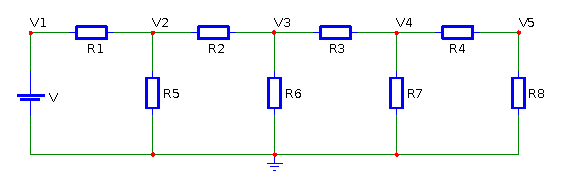
\includegraphics[width=12cm,angle=0]{./cap_linsis/pics/circuito_linear_8.eps}\label{circuitol8}
\end{center}

Complete a tabela abaixo representado a solução com 4 algarismos significativos:

\begin{center}
\begin{tabular}{|c|c|c|c|c|c|}
\hline
Caso & $V_1$ & $V_2$ & $V_3$ & $V_4$ & $V_5$\\
\hline
a & ~\hspace{40pt}~& ~\hspace{40pt}~& ~\hspace{40pt}~& ~\hspace{40pt}~& ~\hspace{40pt}~\\
\hline
b & & & & & \\
\hline
\end{tabular}
\end{center}

Então, refaça este problema reduzindo o sistema para apenas 4 incógnitas ($V_2$, $V_3$, $V_4$ e $V_5$).
\end{exer}
\ifisscilab
\begin{resp}
a)$V_5=98.44V$ b) $V_5=103.4V$

O problema com cinco incógnitas pode ser escrito na forma matricial conforme a seguir:
\begin{equation}\left[\begin{array}{ccccc}
1&0&0&0&0\\[.5cm]
\frac{1}{R_1}&-\left(\frac{1}{R_1}+\frac{1}{R_2}+\frac{1}{R_5}\right)&\frac{1}{R_2}&0&0\\[.5cm]
0&\frac{1}{R_2}&-\left(\frac{1}{R_2}+\frac{1}{R_3}+\frac{1}{R_6}\right)&\frac{1}{R_3}&0\\[.5cm]
0&0&\frac{1}{R_3}&-\left(\frac{1}{R_3}+\frac{1}{R_4}+\frac{1}{R_7}\right)&\frac{1}{R_4}\\[.5cm]
0&0&0&\frac{1}{R_4}&-\left(\frac{1}{R_4}+\frac{1}{R_8}\right)
\end{array}
\right]
\left[\begin{array}{c}
V_1\\[.65cm]
V_2\\[.65cm]
V_3\\[.65cm]
v_4\\[.65cm]
V_5
\end{array}
\right]=
\left[\begin{array}{c}
V\\[.65cm]
0\\[.65cm]
0\\[.65cm]
0\\[.65cm]
0
\end{array}
\right] \end{equation}
Este problema pode ser implementado no \verb+Scilab+ (para o item a) com o seguinte código:
\begin{verbatim}
R1=2, R2=2, R3=2, R4=2, R5=100, R6=100, R7=100, R8=50, V=127

A=[1      0                  0                  0                 0;
   1/R1  -(1/R1+1/R2+1/R5)   1/R2               0                 0;
   0      1/R2              -(1/R2+1/R3+1/R6)   1/R3              0;
   0      0                  1/R3             -(1/R3+1/R4+1/R7)   1/R4;
   0      0                  0                  1/R4             -(1/R4+1/R8)]
v=[V; 0; 0; 0; 0]
y=A\v
\end{verbatim}
O problema com quatro incógnitas pode ser escrito na forma matricial conforme a seguir:
\begin{equation}\left[\begin{array}{cccc}
-\left(\frac{1}{R_1}+\frac{1}{R_2}+\frac{1}{R_5}\right)&\frac{1}{R_2}&0&0\\[.5cm]
\frac{1}{R_2}&-\left(\frac{1}{R_2}+\frac{1}{R_3}+\frac{1}{R_6}\right)&\frac{1}{R_3}&0\\[.5cm]
0&\frac{1}{R_3}&-\left(\frac{1}{R_3}+\frac{1}{R_4}+\frac{1}{R_7}\right)&\frac{1}{R_4}\\[.5cm]
0&0&\frac{1}{R_4}&-\left(\frac{1}{R_4}+\frac{1}{R_8}\right)
\end{array}
\right]
\left[\begin{array}{c}
V_2\\[.65cm]
V_3\\[.65cm]
v_4\\[.65cm]
V_5
\end{array}
\right]=
\left[\begin{array}{c}
-\frac{V}{R1}\\[.65cm]
0\\[.65cm]
0\\[.65cm]
0
\end{array}
\right] \end{equation}
Cuja implementação pode ser feita conforme
\begin{verbatim}
A=[  -(1/R1+1/R2+1/R5)    1/R2               0                 0;
       1/R2              -(1/R2+1/R3+1/R6)   1/R3              0;
       0                  1/R3             -(1/R3+1/R4+1/R7)   1/R4;
       0                  0                  1/R4             -(1/R4+1/R8)]

v=[-V/R1; 0; 0; 0]
y=A\v
\end{verbatim}
\end{resp}
\fi

\begin{exer} Resolva o Problema~\ref{prob_circuito_resistores} pelos métodos de Jacobi e Gauss-Seidel.
\end{exer}


\begin{exer}(Interpolação) Resolva os seguintes problemas:
\begin{itemize}
\item[a)] Encontre o polinômio $P(x)=ax^2+bx+c$ que passa pelos pontos $(-1,-3)$, $(1,-1)$ e $(2,9)$.
\item[b)] Encontre os coeficientes $A$ e $B$ da função $f(x)=A\sin(x)+B\cos(x)$ tais que $f(1)=1.4$ e $f(2)=2.8$.
\item[c)] Encontre a função $g(x)=A_1\sin(x)+B_1\cos(x) + A_2\sin(2x)+B_2\cos(2x)$ tais que $f(1)=1$, $f(2)=2$, $f(3)=3$ e $f(4)=4$.
\end{itemize}
\end{exer}
\begin{resp}
Dica: $P(-1)=-3$, $P(1)=-1$ e $P(2)=9$ produzem três equações lineares para os coeficientes $a$, $b$ e $c$.
Resp: a) $P(x)=3x^2+x-5$, b) $A\approx 2.49$ e $B\approx -1.29$ c)$A_1\approx 1.2872058$, $A_2\approx - 4.3033034$, $B_1\approx 2.051533$ e $B_2\approx - 0.9046921$.
\end{resp}
